\documentclass[11pt]{report}
\usepackage{amsmath}
\usepackage{graphicx}
\usepackage[french]{babel}
\usepackage[utf8]{inputenc}
%\usepackage{fancyhdr}
%\pagestyle{fancy} 
\usepackage[left=2.2cm,right=2.2cm,top=2.5cm,bottom=2.5cm]{geometry}
\usepackage{enumitem}
\usepackage{graphicx}
\usepackage[tikz]{bclogo}
\usepackage{envmath}
\usepackage{amssymb}
\usepackage{array}
\usepackage{multicol}
\usepackage{titlesec, blindtext, color}
\definecolor{gray75}{gray}{0.75}
\newcommand{\hsp}{\hspace{20pt}}
\titleformat{\chapter}[hang]{\huge\bfseries}{\thechapter\hsp\textcolor{gray75}{|}\hsp}{0pt}{\Huge\bfseries}
\titlespacing{\chapter}{0pt}{*0}{*5}
\usepackage{sidecap}
\usepackage{xcolor}
\newcolumntype{C}[1]{>{\centering\arraybackslash }b{#1}}
\usepackage{multirow}


\title{[LICAR1821] Edification Soutenable\\ Synthèse : Hygrothermie, Éclairage et Acoustique}
\date {25 janvier 2017}
\author{Thibaut Heremans\\ Prof.: M. Bodart et M. Vandamme}




\begin{document}
\maketitle
\tableofcontents





\part{Hygrothermie}
\chapter{Flux de chaleur à travers une paroi}
\section{En général}
\paragraph{Hypothèse} On se place dans un contexte de régime stationnaire. C'est à dire que les $T$ et $p$ sont bien établies et constantes dans le temps et qu'il n'y a pas de stockage (chaleur, vapeur d'eau).
\begin{center}
\begin{tabular}{m{2cm}c c}
Position de  & $h_i$  & $h_e$ \\
la paroi et & $ [W/m^2 K]$ & $ [W/m^2 K]$\\
sens du flux & & \\
\hline

\includegraphics[scale=0.07]{mur} & 8 & 23 \\

\includegraphics[scale=0.07]{plafond} & 8 & 23 \\

\includegraphics[scale=0.07]{sol}& 6 & 23\\
\end{tabular}
\end{center}


\begin{center}
\begin{tabular}{lll}
$q$ & $=h_i (\theta_i - \theta_{pi})$ & \; \; \; \; \; \; \; (intérieur)\\
%
 & $= h_e ( \theta_{pe} -  \theta_e)$ & \; \; \; \; \; \; \; (extérieur)\\
 & $=\displaystyle \frac{( \theta_{pi} -  \theta_{pe})}{\sum \frac{d_i}{\lambda_i}}$ & \; \; \; \; \; \; \;  (paroi)\\
\end{tabular}
\end{center}

Le flux de chaleur à travers une paroi s'exprime comme la force motrice globale $\Delta \theta = \theta_i - \theta_e$ divisée par la résistance thermique de la paroi $R_{tot}$ ou multipliée par son coefficient de transmission $U$ :
$$R_{tot} = \frac{1}{h_i}+ \displaystyle \sum \frac{d_i}{\lambda_i} +\frac{1}{h_e} \;\;\;[m^2K/W]\;\;\;\;\;\;\;\;\;\;\;\;\; U= \frac{1}{R_{tot}}$$

$$q=\frac{\theta_i - \theta_e}{R_{tot}} =U(\theta_i - \theta_e) \;\;\;[W/m^2]$$

\section{Cas particuliers}
\subsection*{Lame d'air} Bien que l'air aie un $\lambda_{air} = 0,023 \,W/mK$ , cela ne prend pas en compte les effets de convection et radiation. On utilise plutôt directement $R_a$, sa résistance thermique, donnée dans des tables.

\begin{itemize}
\item Non ventilée : $R_a$ 
\item Peu ventilée :  $\displaystyle \frac{R_a}{2}$
\item Très ventilée : $R_a=0$\\ On admet que $\theta_{air}=\theta_e$ et on néglige tous les matériaux entre la lame d'air et l'extérieur. On rajoute $R_i=\frac{1}{h_i}$ entre la face d'air chaud et la lame elle-même.
\end{itemize}

\subsection*{Paroi en contact avec un local non chauffé} $$R_e = R_i$$
\subsection*{Paroi en contact avec la terre} $$R_e=0$$
\subsection*{Fenêtres} On pondère avec le coefficient du vitrage $U_v$ et  du chassis $U_c$.
$$U_{fen}=\frac{U_v S_v + U_c S_c}{S_v+S_c}\;\;\;[W/m^2K]$$
Par défaut, on prend $S_c = 0,2\, S_{fen}$


\section{Evolution de $\theta$ dans une paroi}
$$\theta_x = \theta_i - R_x \frac{\theta_i - \theta_e}{R_{tot}}\;\;\;[C^{\circ}]$$

\section{Puissance et Energie}
$$P = q S = U \Delta \theta S \;\;\;\; [W]$$
$$Q = P t = U \Delta \theta S t\;\;\;\; [J] \; \textup{ou} \;[Wh]$$

\subsection{Période de chauffe} 
\paragraph{Mise en situation :} Classiquement chez nous, on considère qu'une période de chauffe dure 230 jours avec une température intérieure moyenne $\theta_i=18^{\circ}$ et extérieure $\theta_e=6^{\circ}$. On s'intéresse à l'économie espérée si l'on remplace une fenêtre de $6 \;m^2$ de simple vitrage ($U=6 \;W/m^2K$) par du double vitrage ($U=1,5 \;W/m^2K$).

En appliquant la formule ci-dessus, on obtient $Q_1=2384\;kWh$ (ordre de grandeur) et $Q_2=596\;kWh$. Cela représente donc une économie de $\Delta Q = 1788 \;kWh$. En sachant que la chaleur degagée par $1\;L$ de fuel est de $10\;kWh$, ce sont $179\;L$ qui sont économisés chaque année pour nos $6\;m^2$!




\section{Définitions}
\subsection{Inertie thermique} Capacité d'un matériau à emmagasiner de la chaleur et à ensuite la restituer petit à petit. Cette caractéristique est très importante pour garantir un bon confort notamment en été, c'est-à-dire pour éviter les surchauffes.\\

Elle permet de limiter les effets d'une variation "rapide" de la température extérieure sur le climat intérieur par un déphasage entre la température extérieure et la température de surface intérieure des murs et par amortissement de l'amplitude de cette variation. Un déphasage suffisant permettra par exemple que la chaleur extérieure "n'arrive" qu'en fin de journée dans l'habitat, période où il est plus facile de le rafraîchir grâce à une simple ouverture des fenêtres.


\begin{figure}[h]
\begin{center}
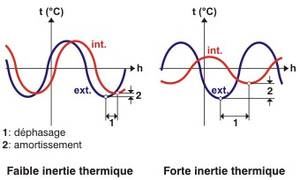
\includegraphics[width=0.5\linewidth]{RTEmagicC_Inertie_thermique_-_dephasage_et_amortissement.jpg}
%\caption{Déphasages entre $T_e$ et $T_i$}
\end{center}
\end{figure}



\subsection{Pont thermique}
Les ponts thermiques sont des points faibles dans l'isolation thermique de l'enveloppe du bâtiment.
À ces endroits, en hiver, la température superficielle de l'enveloppe est plus basse que celle des surfaces environnantes.
Ils découlent, en général de contraintes constructives ou géométriques
et vont provoquer des dépenses énergétiques, un inconfort sur le plan de l'hygiène et la détérioration des matériaux.


\subsubsection{Pont thermique dû à des contraintes constructives}
\begin{minipage}{0.3\linewidth}
\centering
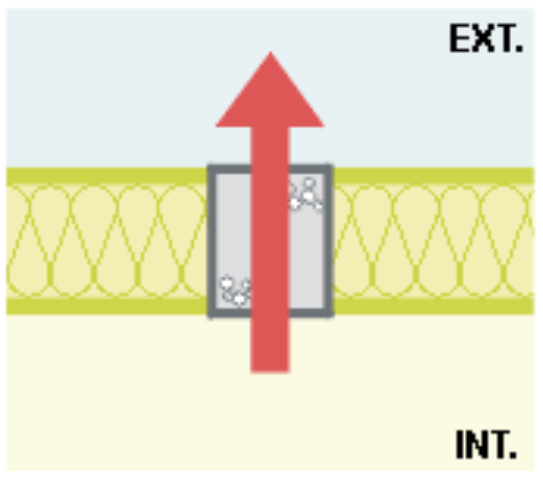
\includegraphics[scale=0.4]{pont1}
\end{minipage}
\begin{minipage}{0.65\linewidth}
Les matériaux isolants ont généralement des capacités limitées en matière de résistance aux contraintes mécaniques. Le principe de la continuité de la couche isolante n'a pas été respecté, ou n'a pu l'être dans certains cas, à certains endroits.\\

 Il s'agit par exemple d'ancrages ou d'appuis entre d'éléments situés de part et d'autre de la couche isolante de la paroi. L'isolant étant localement absent, le flux de chaleur est sensiblement plus dense dans ces parties de la paroi.
\end{minipage}


\subsubsection{Pont thermique dû à des contraintes géométriques}
\begin{minipage}{0.3\linewidth}
\centering
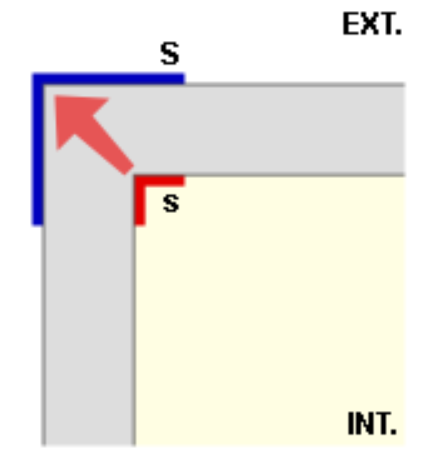
\includegraphics[scale=0.45]{pont2}
\end{minipage}
\begin{minipage}{0.65\linewidth}
Ce type de pont thermique est dû à la forme de l'enveloppe à un endroit. A cet endroit, la surface de la face extérieure (surface de refroidissement) est beaucoup plus grande que la surface de la face intérieure (surface chauffée).

\end{minipage}







\newpage
\chapter{Flux de vapeur d'eau à travers une paroi}
\section{En général}
%\begin{center}
%\begin{tabular}{lcc}
%Grandeur & symbole & unités \\
%\hline
%Humidité absolue de l'air & $x$ & $[g/kg]$ \\
%Humidité absolu de l'air saturé & $x_s$ & $[g/kg]$ \\
%Pression partielle de vapeur  & $p$ & $[Pa]$\\
%Pression de saturation de vapeur & $p_s$ & $[Pa]$\\
%Humidité relative de l'air & $\phi$ & [\%]\\
%Température de rosée & $T_r$ & $[C^{\circ}]$\\
%Masse volumique de l'air & $\rho$ & $[kg/m^3]$\\
%\end{tabular}
%\end{center}

L'humidité relative $\phi$ se défini comme le rapport de l'humidité absolue (cfr. pression partielle) de l'air sur son humidité (cfr. pression) saturée :
$$\phi \triangleq \frac{x}{x_s}.100= \frac{p}{p_s}.100\;\;\;[\%] $$

De manière analogue au flux de chaleur, le flux de vapeur à travers une paroi, s'exprime comme la force motrice globale $\Delta p = p_i - p_e$ divisé par le coefficient de résistance à la diffusion de vapeur d'eau de la paroi $Z_{tot}$.

$$Z_{tot} = C \sum \mu_i d_i \;\;\;[m/s]\;\;\;\;\;\;\;\;\;\;\; \textup{avec}\;\;\ C=5,4 \,10^9\, [s^{-1}]$$

$$q_v = \frac{p_i - p_e}{Z_{tot}}\;\;\;[kg/m^2 s]$$

Où $\mu \triangleq \displaystyle \frac{C_{mat}}{C_{air}}$ ce que implique que $\mu_{air}=1$. Le verre étant un matériaux non poreux, $\mu_{verre}= \infty$. \\

%Attention au fait que tous les isolants, à $\lambda$ égaux, n'ont pas le même comportement face à la vapeur d'eau. 
%\begin{center}
%\begin{tabular}{lcl}
%\textbf{Isolant} & $\mu\,d$ & \textbf{Comportement}\\
%\hline
%Laine de verre & $0,15$ & Traverse facilement\\
%Verre cellulaire & $\infty$ & Imperméable\\
%Mousses synthétiques & $30$ & Traverse difficilement\\
%\end{tabular}
%\end{center}

\section{Cas particuliers}
\subsection*{Lame d'air}
\begin{itemize}
\item Non ventilée : Calcul normal avec $\mu_{air}=1$
\item Ventilée : On admet que $p_{air}=p_e$ et on néglige tous les matériaux entre la lame d'air et l'extérieur.
\end{itemize}


\section{Évolution de $p$ dans une paroi}
$$p_x = p_i - Z_x \frac{p_i - p_e}{Z_{tot}}\;\;\;[Pa]$$



\section{Condensation superficielle}
En diminuant la température de l'air, on peut le saturer de vapeur d'eau ($T < T_{ros\acute{e}e}$). C'est notamment ce qui se passe en hiver  sur les fenêtres, surfaces plus froides que le local. Étant donné que $\mu_{verre}= \infty$, l'eau ne traverse pas et ne fait que couler sur la vitre. Dans le cas d'un mur c'est plus problématique. Si une condensation superficielle se forme régulièrement sur un mur (surface poreuse), les matériaux qui le composent s'humidifient sur une certaine profondeur. Il n'y a pas de soucis tant que le condensat arrive à sécher (notons que $t_{dry} = 10 . t_{hum}$). Sinon il peut y avoir des dégâts.

Si l'on veut éviter ce phénomène, il faut veiller à ce qu'aucun matériau n'ait une température superficielle inférieure au point de rosée de l'air du local. Il suffit alors d'augmenter la température de surface des parois (\textbf{chauffer\footnote{Attention, aux endroits où les échanges de chaleur se font plus difficilement (coins, derrières meubles, ...) Leur $h_i$ diminue et donc leur $T_{pi}$ aussi.} ou isoler}) ou de diminuer la teneur en humidité de l'air (\textbf{ventiler}\footnote{Ramener de l'air sec de dehors, le chauffer pour qu'il puisse enmagasiner plus de vapeur et puis le rejeter dehors.}).


\section{Condensation interne}
Pour déterminer s'il y a condensation interne, il faut calculer les température à chaque interface dans le mur. Pour chacune de ces température, le tableau des $p_s$ permet de trouver $p$. Si la courbe de $p$ (linéaire) coupe celle de $p_s$, il a condensation.

\subsection{Méthode de Glaser}
Glaser a formulé l'hypothèse suivante : L'évolution de $p$ doit passer par $p_{sc}$, la pression de saturation du lieu où il y a la plus forte condentation (le plus grand écart entre $p$ et $p_s$). Il propose de tracer les droites ($p_i,p_{sc}$) et ($p_{sc},p_e$) comme représentatives des flux entrant et sortant réels.

\begin{figure}[h]
\begin{center}
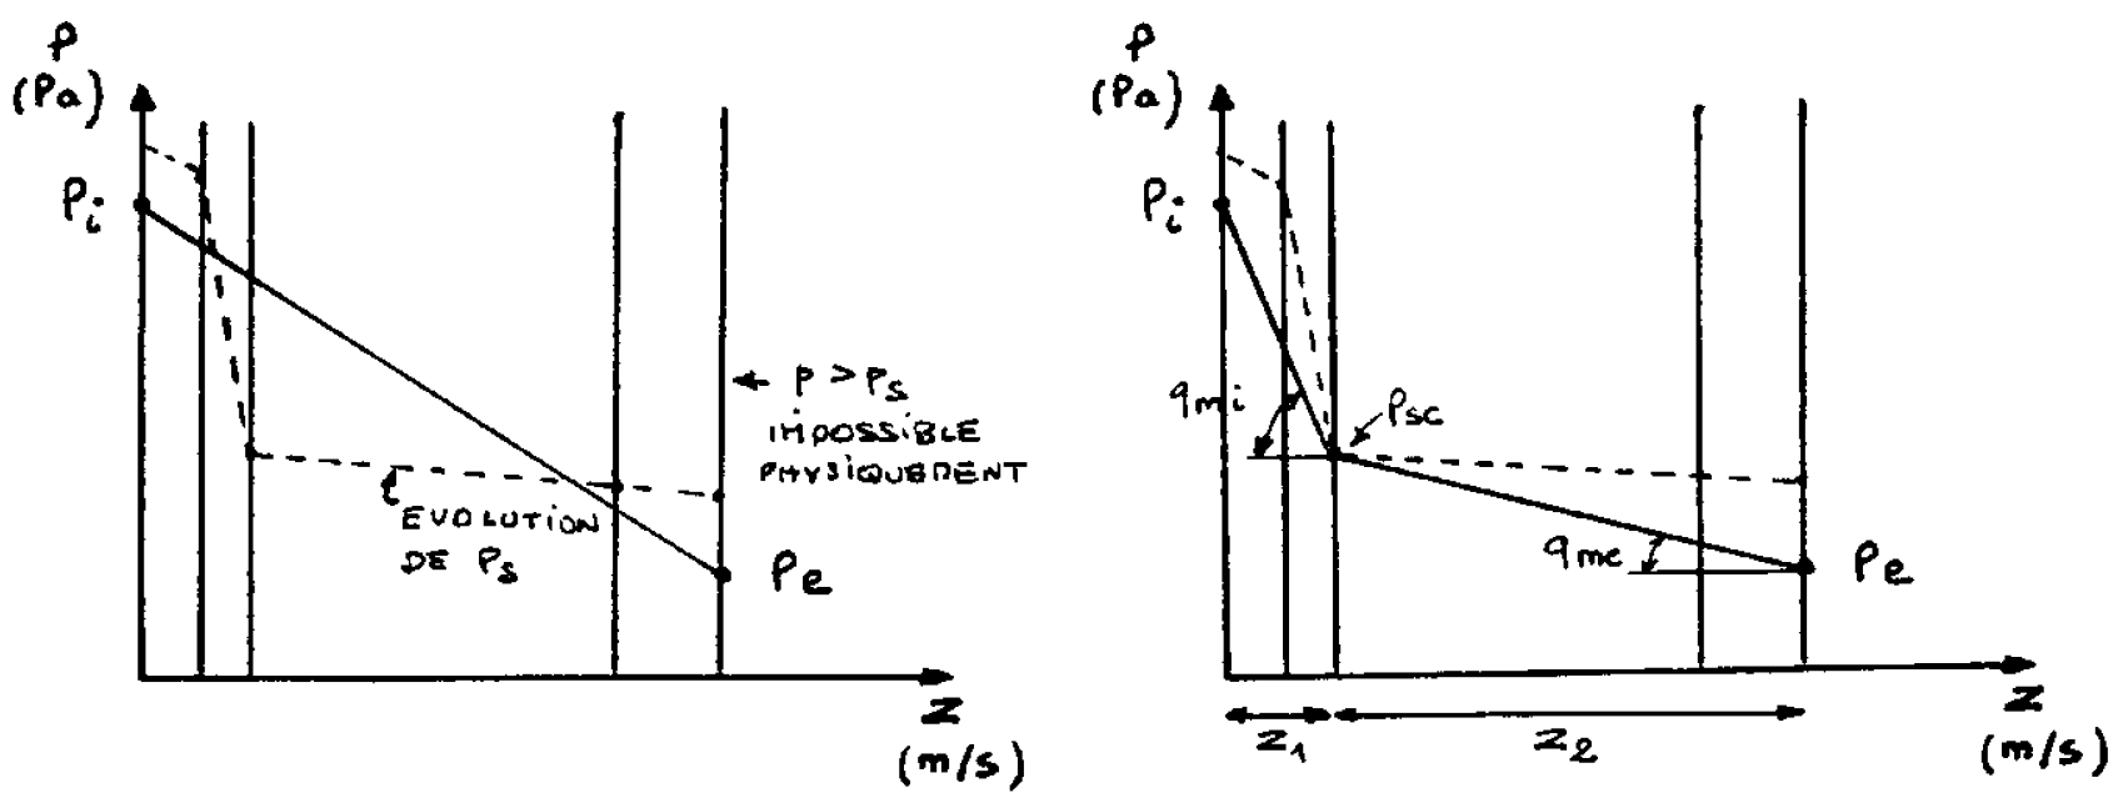
\includegraphics[width=\linewidth]{pp}
\end{center}
\caption{Méthode graphique de Glaser}
\end{figure}

La quantité de condensat est égal à la différence entre le flux entrant et sortant (régime stationnaire). 
$$q_{mc}=q_{mi}-q_{me} = \frac{p_i-p_{sc}}{Z_1}-\frac{p_{sc}-p_e}{Z_2}\;\;\;[kg/m^2 s]$$

Pour éviter les problèmes de condensation interne, on place de préférence le pare-vapeur du côté chaud (intérieur) de l'élément de construction et l'isolant à l'extérieur.


\newpage
\section{Diagramme de Mollier}
\begin{figure}[!h]
\centering
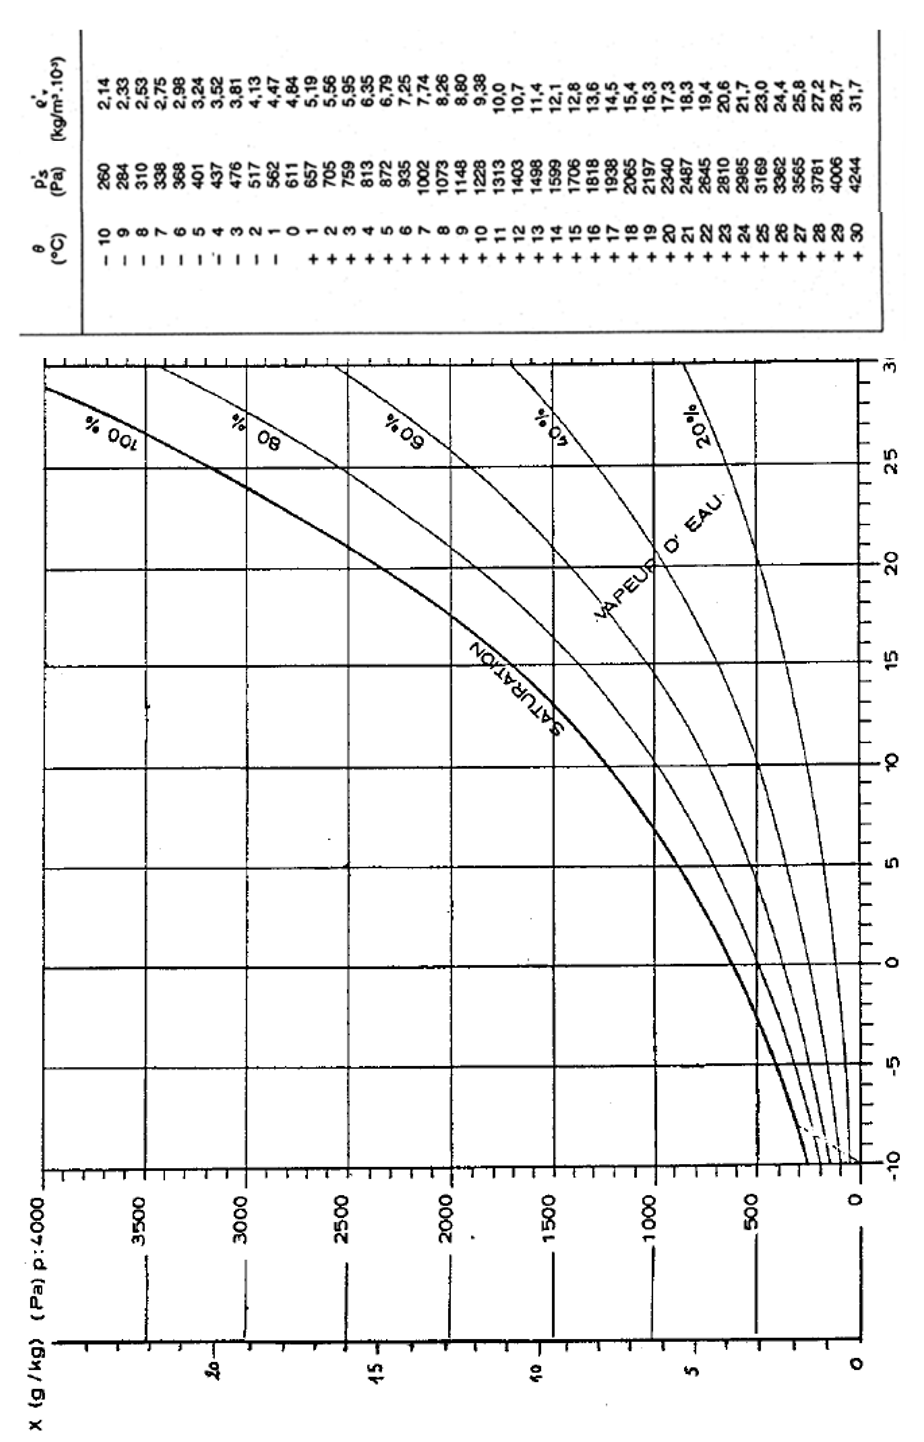
\includegraphics[width=0.8\linewidth]{tot}
%\caption{Exemple de luminaires de chez DMLights}
\end{figure}








\part{Éclairage}
\chapter{Notions Fondamentales}
\section{Grandeurs relatives au rayonnement}
\subsection{Double système d'unité}
On peut considérer les grandeurs relatives au rayonnements sous deux aspects.

\begin{center}
\begin{tabular}{l|cc}
 &  \textbf{Physique} & \textbf{Physiologique}\\ 
 Domaine & Radiométire & Photométrie\\
Phénomène & Transport d'énergie & Sensations visuelles\\
Caractéristique & Spectre EM complet & Restreint au spectre visible\\
Notation & Indice $e$ & Pas d'indice\\
\end{tabular}
\end{center}

Les deux points de vue sont reliés par la relation de proportionnalité suivante pour une grandeur $G$ quelconque
$$G = K_M \int_0^{\infty} V(\lambda) G_{e\lambda} d\lambda$$

avec $K_m = 683 \; [lm/W]$ le facteur de proportionnalité, $V(\lambda)=0$ en dehors du visible, le facteur qui restreint le spectre au visible et $G_{e\lambda}$ la densité spectrale énergétique. Toutes les grandeurs définies ci-après possède un équivalent énergétique et lumineux.

\subsection{Flux}
\begin{minipage}{0.2\linewidth}
\centering
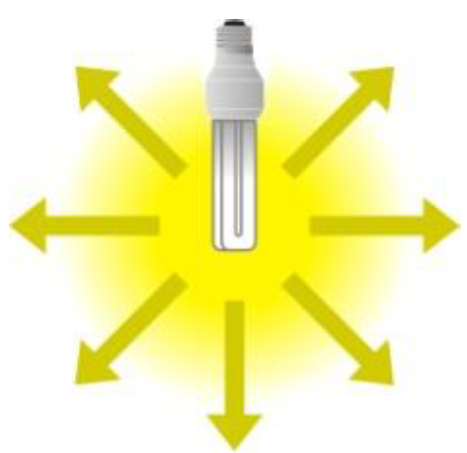
\includegraphics[scale=0.2]{flux}
\end{minipage}
\begin{minipage}{0.75\linewidth}
Le flux énergétique $\phi_e$ ou lumineux $\phi$ est la quantité totale d'énergie ou de lumière émise par la source par unité de temps dans toutes les directions, $[W]$ ou $[lm]$.
\end{minipage}


\subsection{Intensité}
\begin{minipage}{0.2\linewidth}
\centering
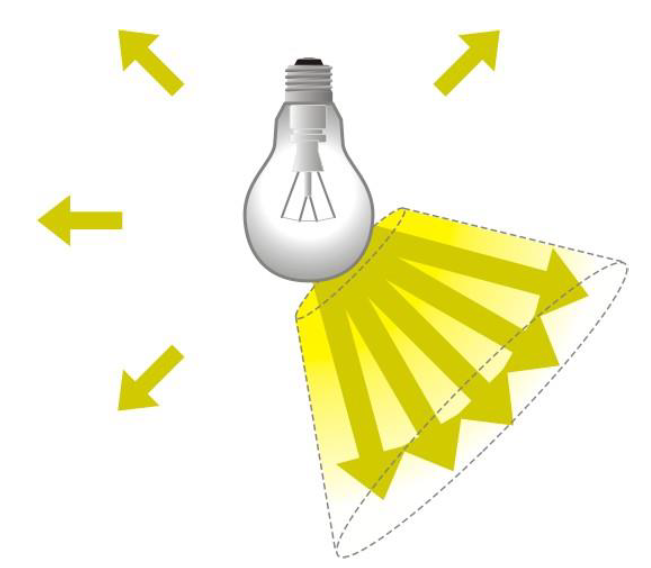
\includegraphics[scale=0.2]{intensite}
\end{minipage}
\begin{minipage}{0.75\linewidth}
L'intensité est une grandeur directionnelle (vectorielle) et n'a donc de sens que pour une source ponctuelle. On considère une source comme ponctuelle dès que l'on se trouve à une distance d'observation 5-10 fois supérieure à la plus grande longueur de la source.
\end{minipage}

\vspace{5mm}
\textbf{Notion d'angle solide :} Noté $\Omega$ ou $\omega$ c'est un angle en 3D qui mesure la grandeur apparente sous laquelle un objet apparait à un observateur. Pour une surface $S$ située à une distance $R$, un angle solide est défini par
$$\omega = \frac{S}{R^2} \;\;\;\;\;\;\;\; [sr]$$ 

L'intensité énergétique $[W/sr]$ ou lumineuse $[lm/sr]\triangleq[cd]$ dans la direction $A$ est alors le rapport du flux respectif par unité d'angle solide
$$I_A = \frac{d\phi}{d\omega}\;\;\;\;\;\;\;\; [W/sr]\;\;\;\;\textup{ou} \;\;\;\; [cd]$$

\vspace{5mm}
\textbf{Application :} On peut représenter l'intensité lumineuse d'une source (lampe + luminaire) dans différentes directions sous forme d'un diagramme polaire. Il permet de voir facilement comment la lumière d'une source sera dirigée. Dans les fiches techniques, les fabricants superposent deux traits, rouge et bleu ci-dessous, qui représentent la distribution dans l'axe [$90-270^{\circ}$] et perpendiculaire à la lampe [$180^{\circ}$], respectivement. 


\begin{figure}[h]
\begin{minipage}{0.7\linewidth}
\centering
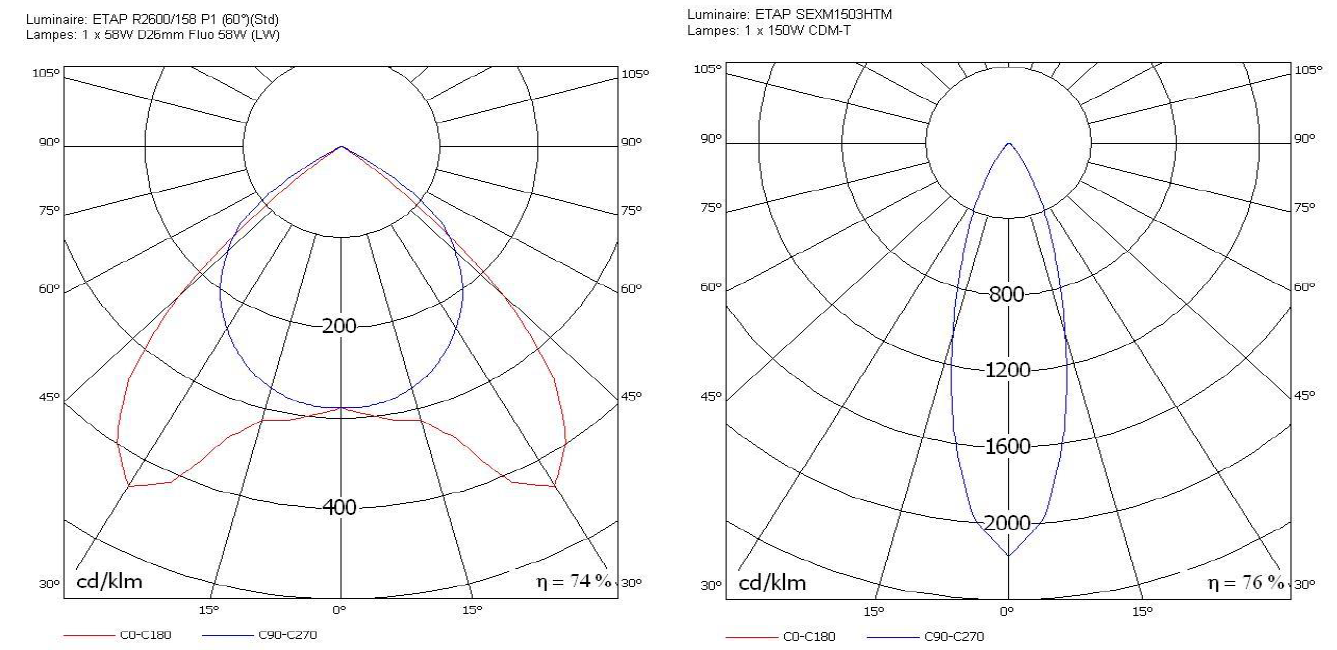
\includegraphics[width=\linewidth]{polaire}
\end{minipage}
\begin{minipage}{0.28\linewidth}
\centering
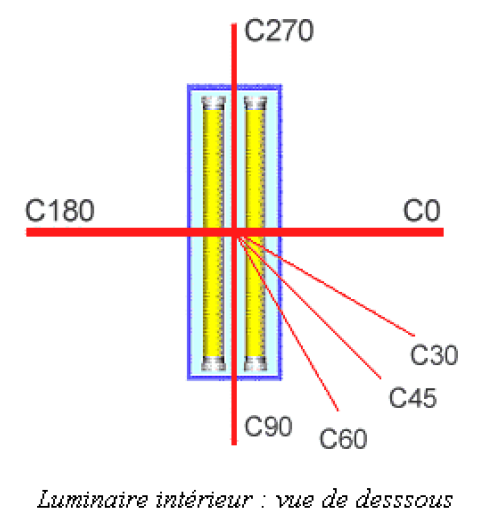
\includegraphics[width=\linewidth]{diagcd}
\end{minipage}
\caption{A gauche, une source intensive selon son axe et extensive perpendiculairement (tube fluorescent). A droite, une source intensive dans les deux directions (spot)}
\end{figure}

Consulter l'Annexe \ref{an1} pour plus d'exemples.


%
%\begin{figure}[h]
%\centering
%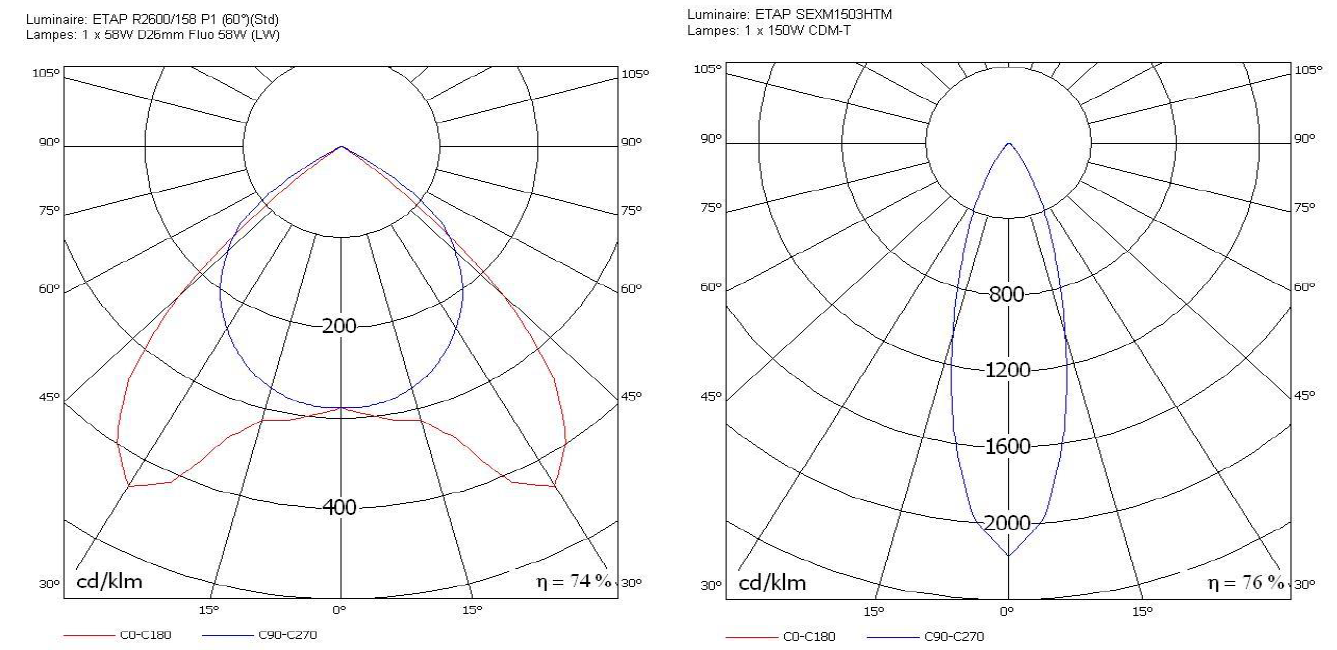
\includegraphics[width=0.7\linewidth]{polaire}
%\caption{A gauche, une source extensive selon son axe et intensive perpendiculairement (tube fluorescent). A droite, une source intensive dans les deux directions (spot)}
%\end{figure}



\subsection{Éclairement}
\begin{minipage}{0.2\linewidth}
\centering
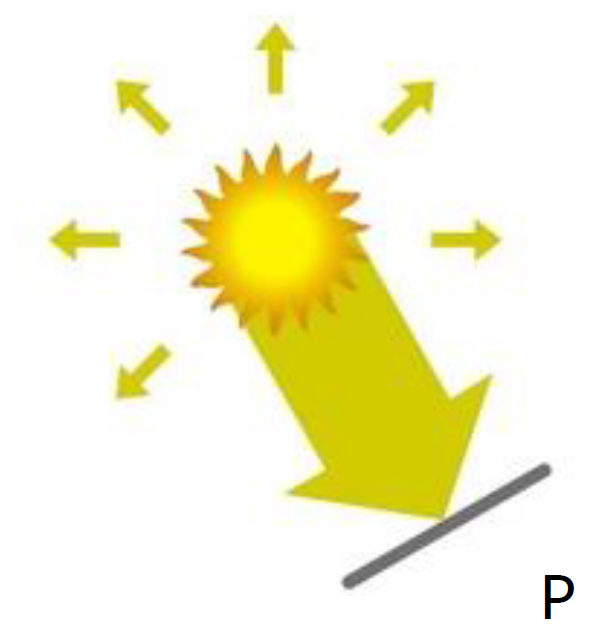
\includegraphics[scale=0.2]{eclair}
\end{minipage}
\begin{minipage}{0.75\linewidth}
Contrairement aux deux grandeurs précédentes,c'est une caractéristique de la surface éclairée et non de la source.\\ L'éclairement énergétique $[W/m^2]$ ou lumineux $[lm/m^2]\triangleq[lx]$ d'une surface $dS$ en un point $P$ est défini comme le rapport entre le flux reçu et la surface lorsque $dS \longrightarrow 0$.
$$E_P = \frac{d\phi}{dS}\;\;\;\;\;\;\;\; [W/m^2]\;\;\;\;\textup{ou} \;\;\;\; [lx]$$
\end{minipage}


\subsection{Luminance}
\begin{minipage}{0.2\linewidth}
\centering
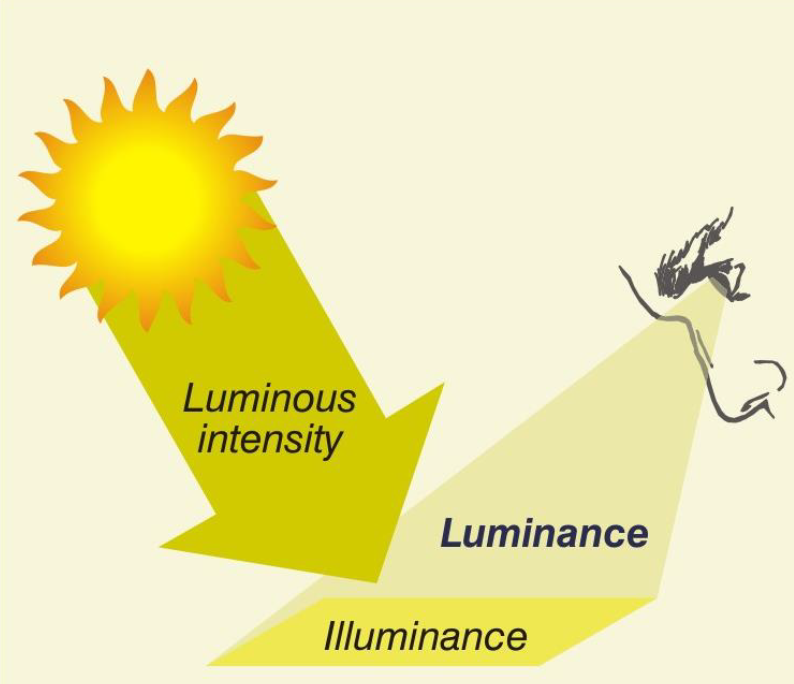
\includegraphics[scale=0.18]{lumi}
\end{minipage}
\begin{minipage}{0.75\linewidth}
La luminance est définie à partir de l'intensité et est donc aussi une grandeur vectorielle. Elle traduit pour un point $P$ de la surface émissive, l'intensité par unité de surface apparente dans la direction $A$.
C'est elle qui caractérise l'aspect visuel de ce qui nous entoure. Elle est liée aux notions de brillance, d'éclat et de luminosité.
\end{minipage}


\begin{minipage}{0.3\linewidth}
\centering
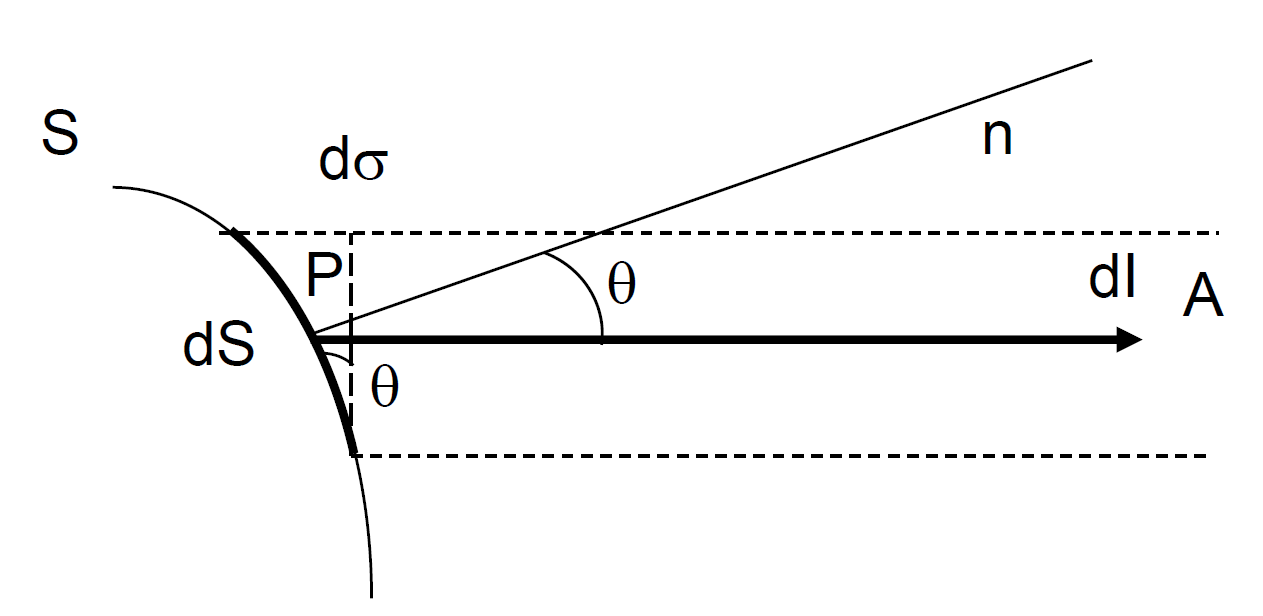
\includegraphics[scale=0.22]{lumi_dia}
\end{minipage}
\begin{minipage}{0.65\linewidth}
$$L_{P,A} = \frac{dI}{dS cos \theta}\;\;\;\;\;\;\;\; [W/sr m^2]\;\;\;\;\textup{ou} \;\;\;\; [cd/m^2]$$

\end{minipage}



\newpage
\subsection{Appareils de mesures}
On utilise un luxmètre pour mesurer l'éclairement (gauche) et un  luminancemètre pour la luminance (droite).

\begin{minipage}{0.5\linewidth}
\centering
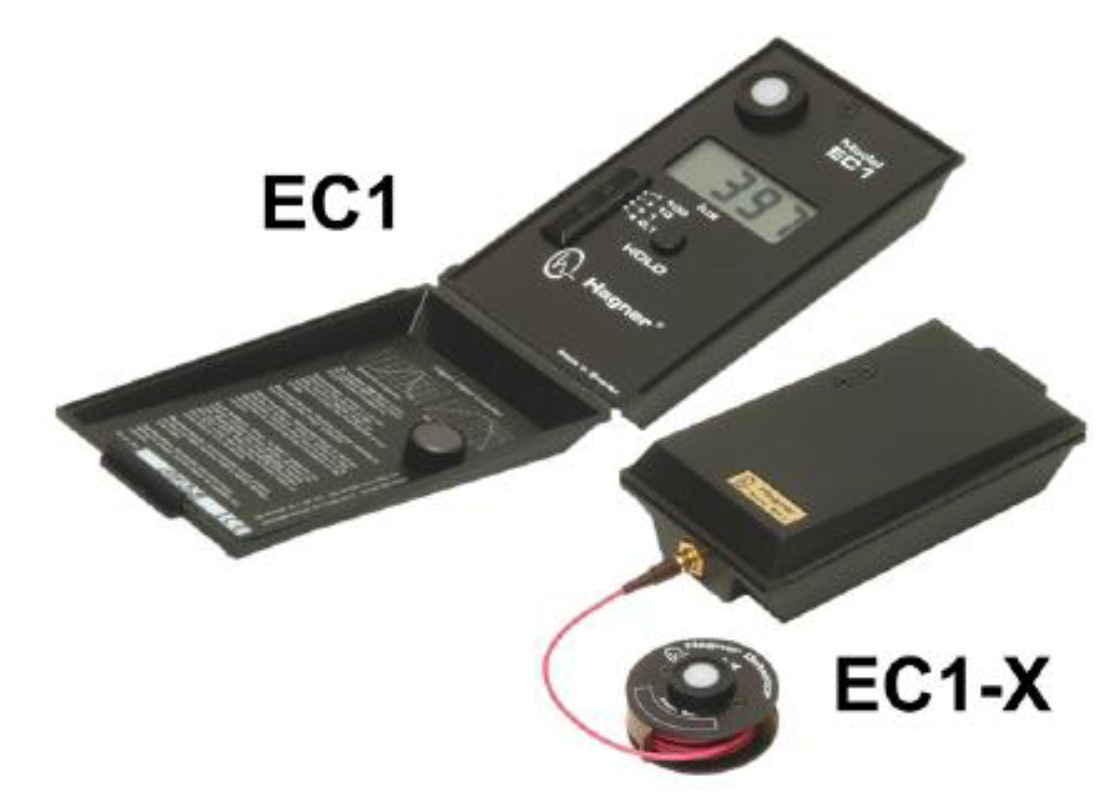
\includegraphics[width=0.3\linewidth]{luxm}
\end{minipage}
\begin{minipage}{0.5\linewidth}
\centering
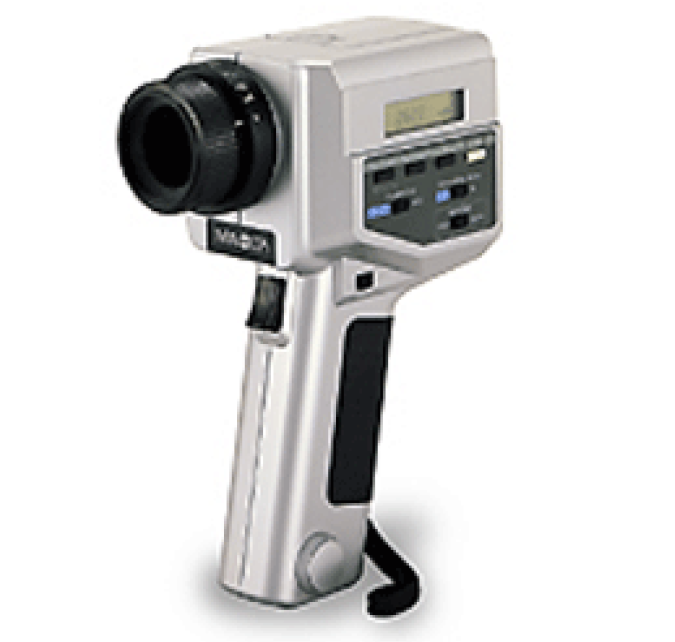
\includegraphics[width=0.3\linewidth]{lumm}
\end{minipage}



\subsection{Ordres de grandeur}
\begin{tabular}{m{3.5cm}m{13cm}}
Flux $[lm]$ & 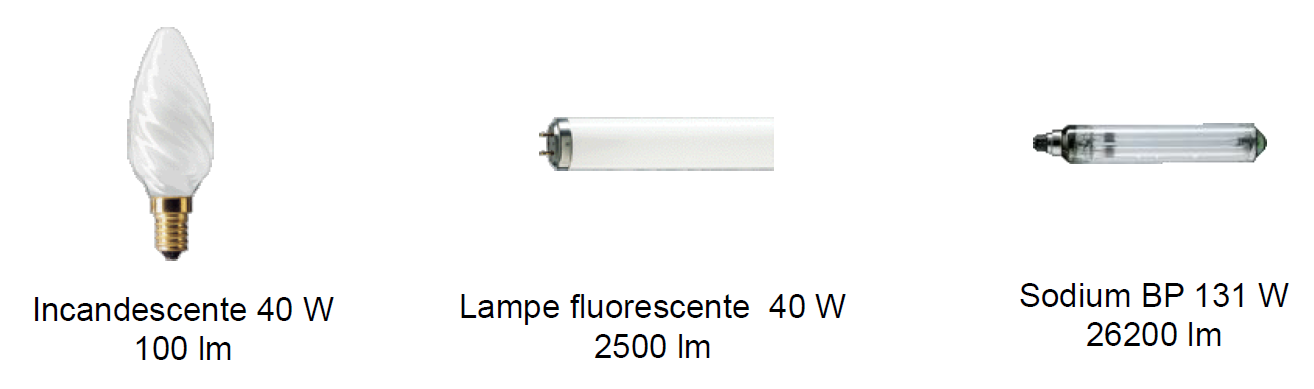
\includegraphics[scale=0.4]{lm} \\
Angle solide $[sr]$ & 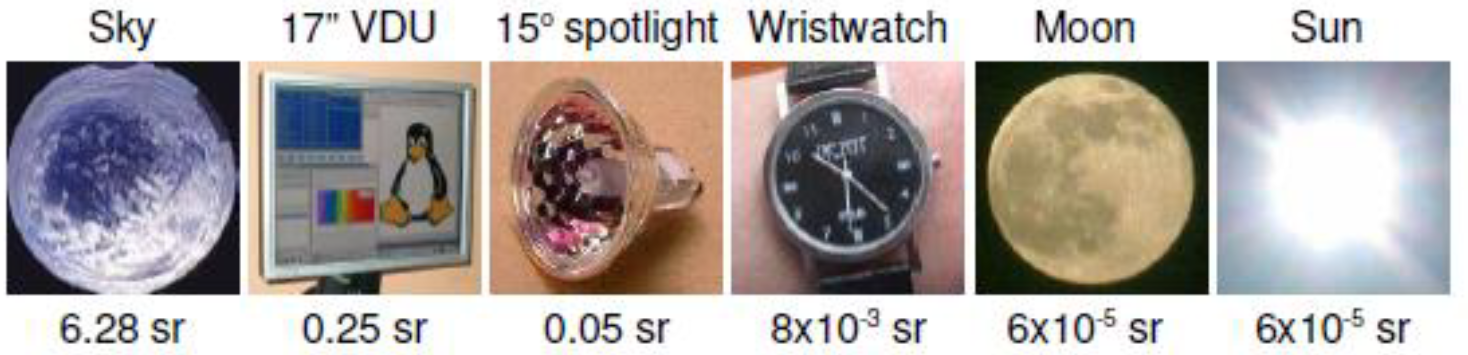
\includegraphics[scale=0.4]{sr} \\
Intensité $[cd]$ & 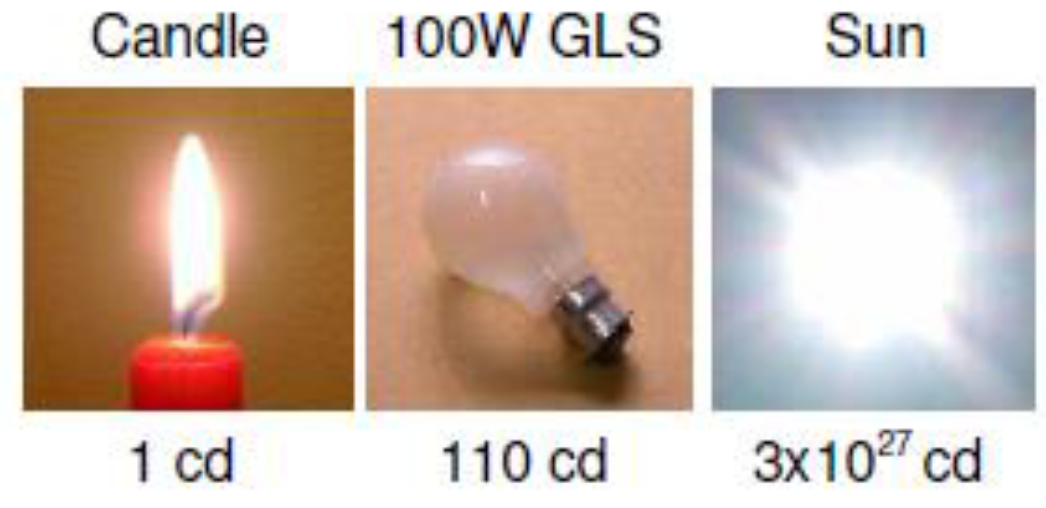
\includegraphics[scale=0.3]{cd} \\
Éclairement $[lx]$ & 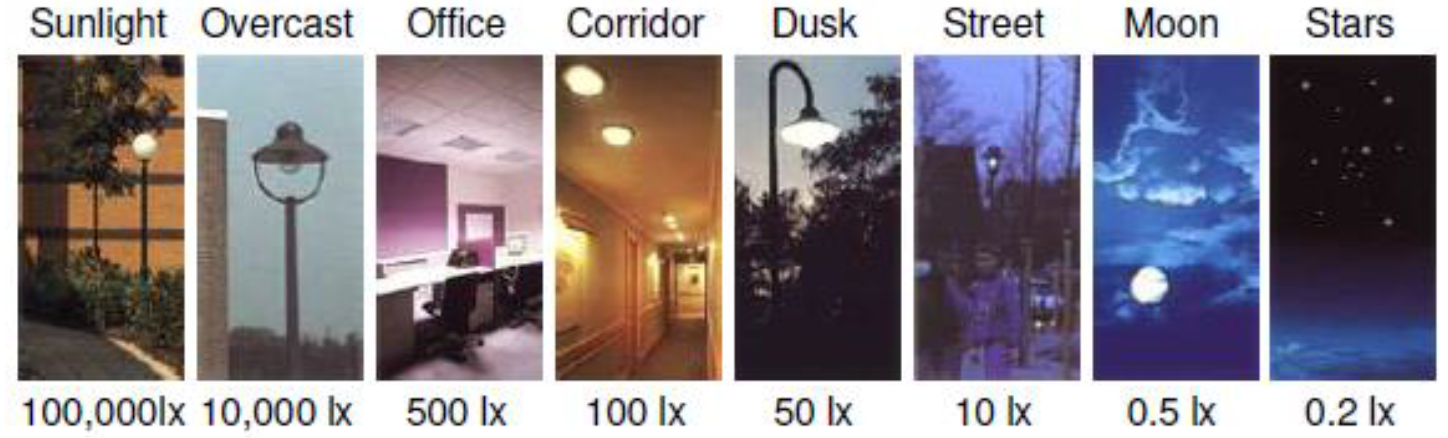
\includegraphics[scale=0.35]{lux}\\
Luminance $[cd/m^2]$ & 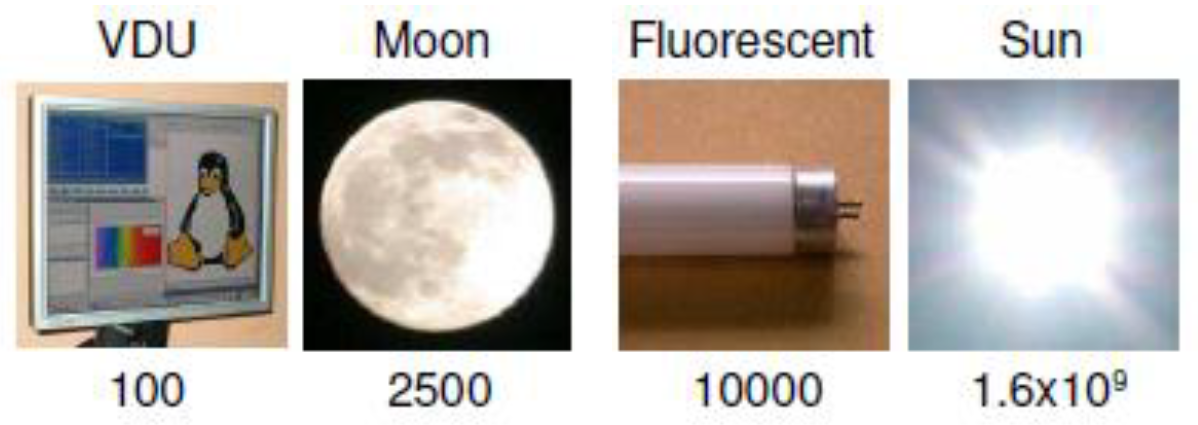
\includegraphics[scale=0.35]{cdm2} \\
\end{tabular}


%TABLEAU RECAP??








\section{Lois générales de la technique de l'éclairage}
\subsection{Relation intensité-éclairement}
\begin{minipage}{0.4\linewidth}
$$E_P = \frac{I \, \cos \theta}{D^2}$$
L'éclairement varie en $\displaystyle \frac{1}{D^2}$ et est proportionnel a $\cos \theta$.
\end{minipage}
\begin{minipage}{0.6\linewidth}
\centering
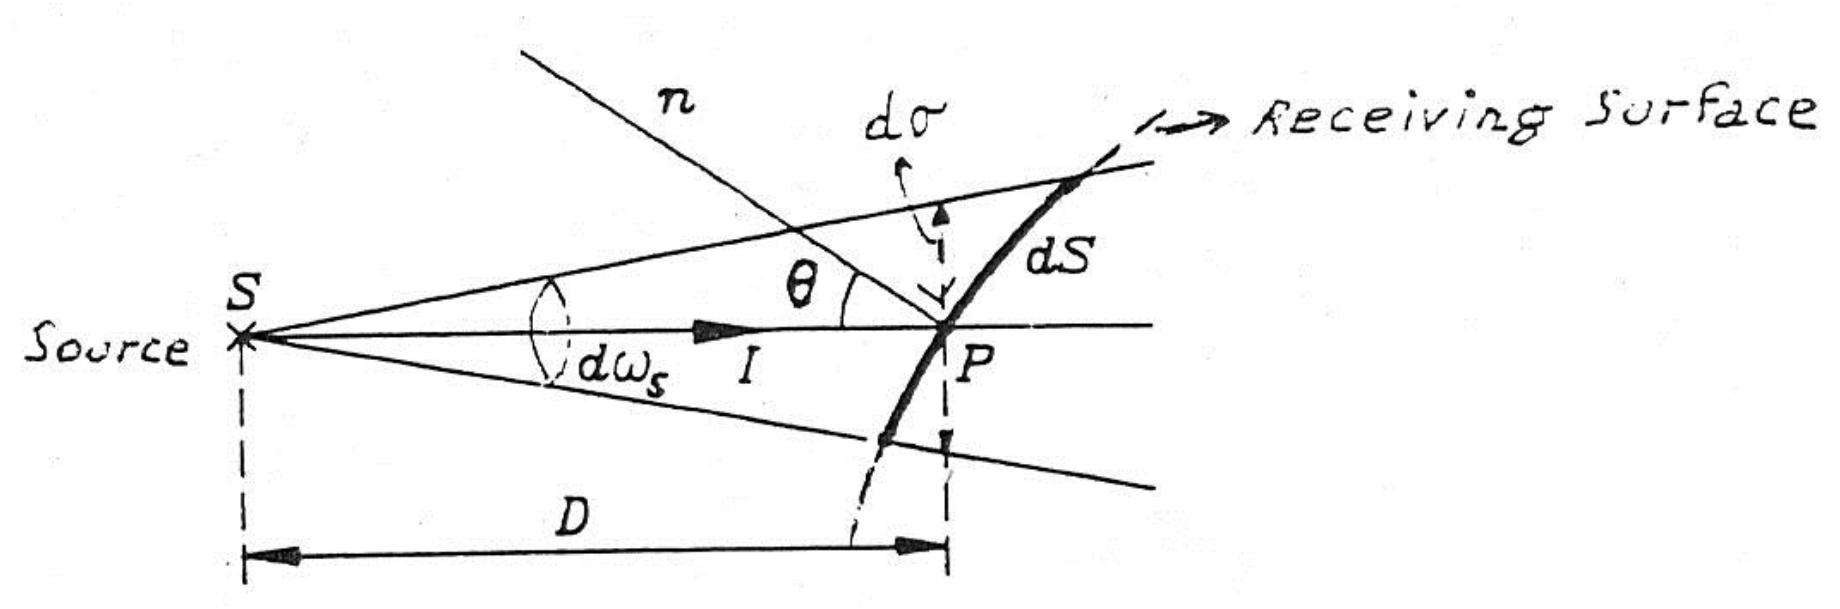
\includegraphics[width=0.9\linewidth]{inversedist}
\end{minipage}


\subsection{Loi de Lambert pour les sources orthotropes}
\begin{minipage}{0.4\linewidth}
\centering
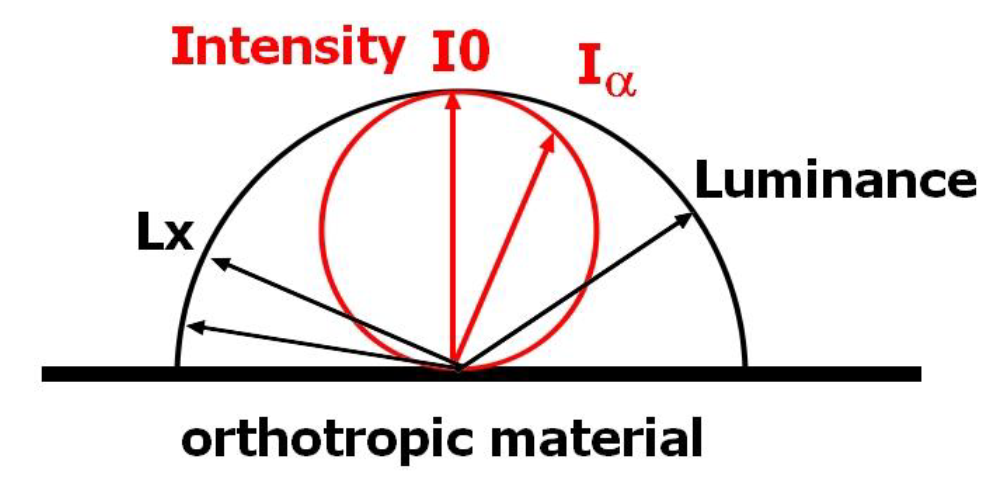
\includegraphics[scale=0.3]{lambert}
\end{minipage}
\begin{minipage}{0.6\linewidth}
Une source orthotrope (lambertienne) est une source primaire ou un corps diffusant qui émet/renvoie de la lumière avec une luminance constante dans toutes les directions de l'hémisphère du point considéré (ex: neige, brouillard, peinture mat).
\end{minipage}


\vspace{1cm}
La loi de Lambert relie la luminance à l'éclairement. C'est une formule très pratique car la luminance est un paramètre significatif de l'impression visuelle mais difficile à mesurer alors que l'éclairement, lui, se mesure facilement.

$$L = \frac{\rho}{\pi}E$$
où $\rho$ est le coefficient de réflexion (voir section \ref{reflex}). 






\newpage
\section{Propriétés optiques des matériaux}
\label{reflex}
\begin{minipage}{0.4\linewidth}
\centering
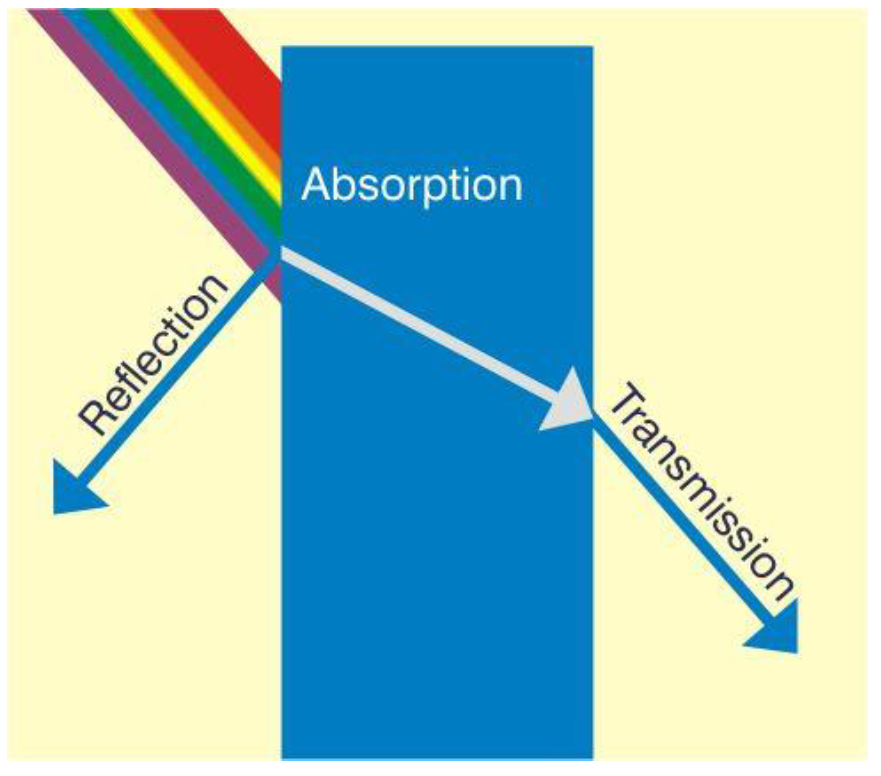
\includegraphics[scale=0.3]{prop}
\end{minipage}
\begin{minipage}{0.6\linewidth}
Lorsqu'un flux de lumière  incident $\phi_i$ arrive sur une surface, il a 3 modes de propagation : être réfléchi, absorbé ou transmis. Chacun de ces modes est défini par son coefficient.
\begin{itemize}
\item \textbf{Coefficient de réflexion :} $\rho= \frac{\phi_r}{\phi_i}$
\item \textbf{Coefficient d'absorption :} $\alpha= \frac{\phi_t}{\phi_i}$
\item \textbf{Coefficient de transmission :} $\tau= \frac{\phi_t}{\phi_i}$
\end{itemize}
$$\rho + \alpha + \tau = 1$$
\end{minipage}


\subsection{Réflexion}
La réflexion est fonction de la brillance de la surface. 
\begin{itemize}
\item Spéculaire (miroir, métal poli) : réflexion parfaite
\item Brillante : réflexion partielle
\item Mat : Diffusion parfaite
\item Satin : réflexion parfaite pour des grands angles d'incidence $i$ et diffusion parfaite pour des petits $i$.
\end{itemize}
\begin{SCfigure}[20][h]
\centering
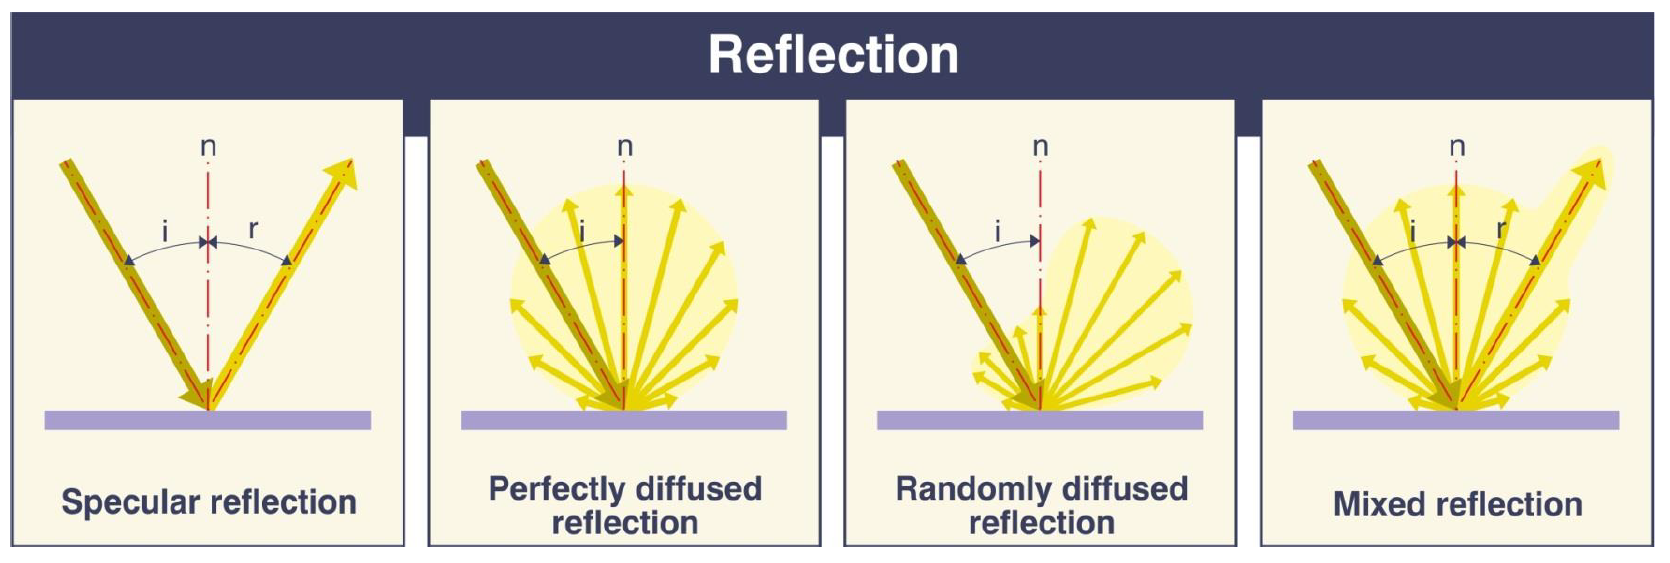
\includegraphics[width=0.72\linewidth]{refle}
\caption{Types de réflexion}
\end{SCfigure}



\subsection{Transmission}
La transmission est fonction de l'épaisseur. On distingue les matériaux transparents ($\tau \simeq 1$), des matériaux translucides ($0 < \tau < 1$) et des matériaux opaques ($\tau \simeq 0$). 
\begin{SCfigure}[20][h]
\centering
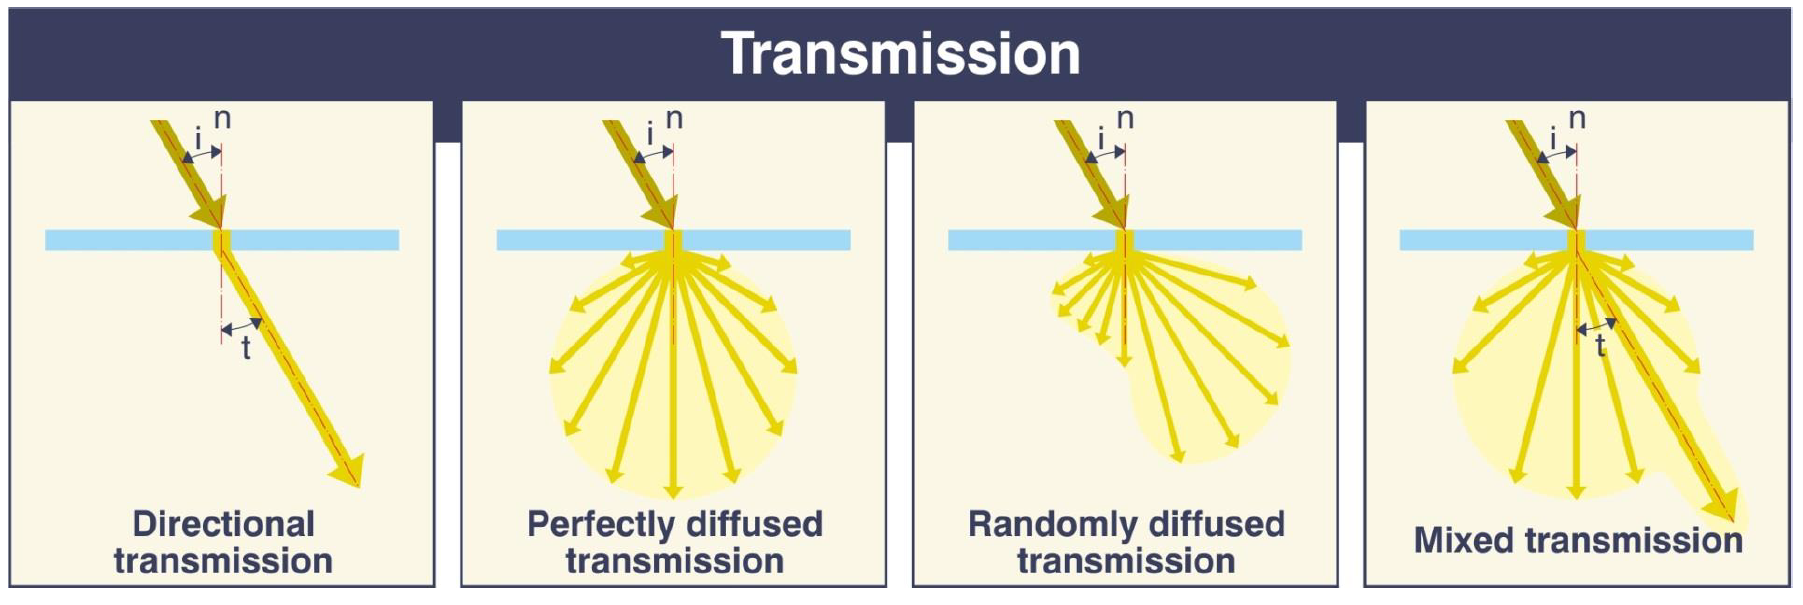
\includegraphics[width=0.72\linewidth]{trans}
\caption{Types de transmission}
\end{SCfigure}



\subsection{Perception des couleurs}
La couleur est une sensation visuelle subjective. L'œil interprète un stimulus (spectre de réflexion de l'objet). Comparons les spectres d'une pomme et d'un citron. 

\begin{minipage}{0.5\linewidth}
\centering
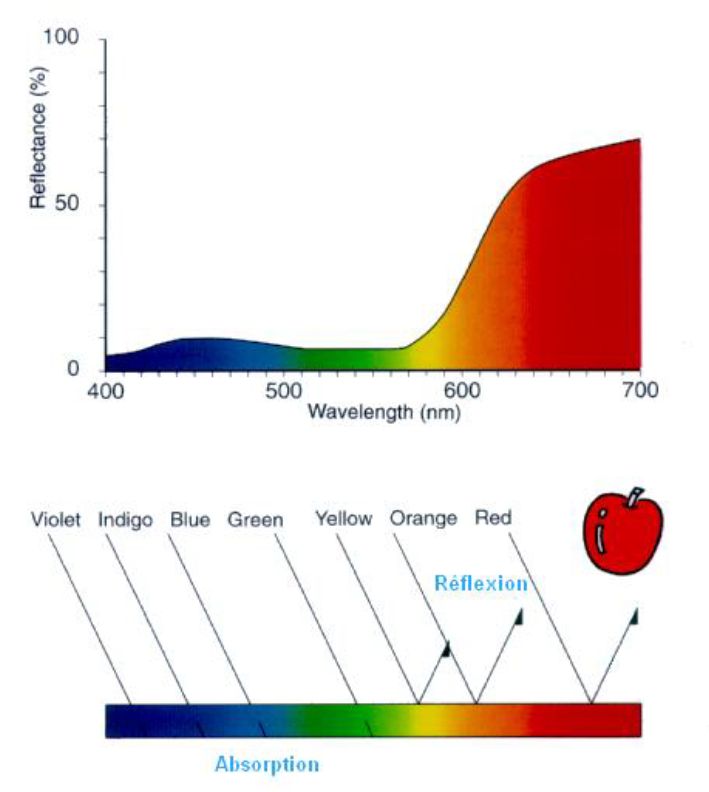
\includegraphics[width=0.8\linewidth]{pom}
\end{minipage}
\begin{minipage}{0.51\linewidth}
\centering
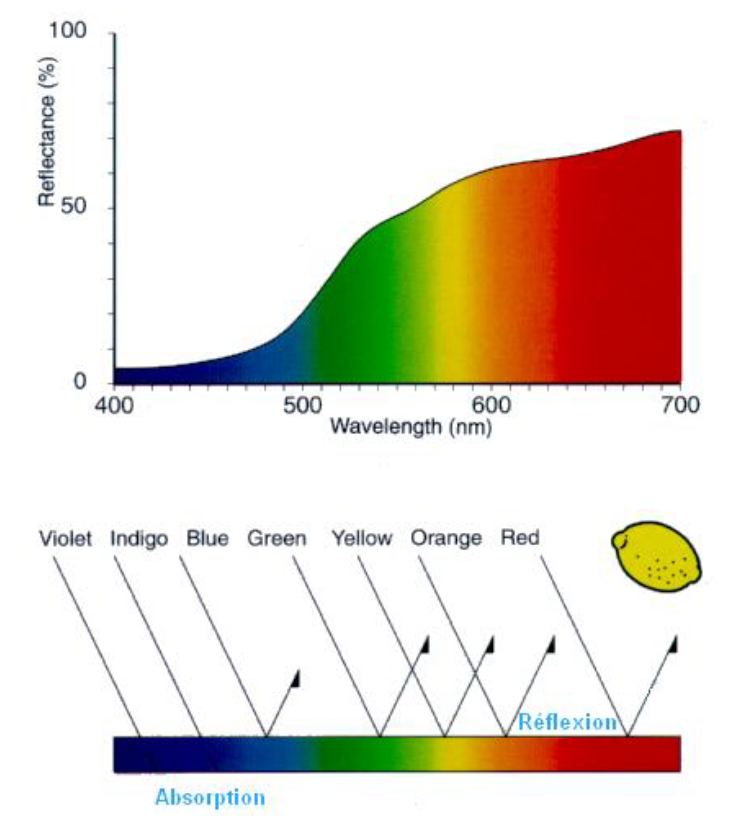
\includegraphics[width=0.8\linewidth]{citron}
\end{minipage}

\vspace{5mm}
Les deux spectres sont relativement similaires alors que les couleurs finales sont radicalement différentes. C'est dû au fait que l'œil humain ne réagit pas de la même manière pour toutes les longueurs d'ondes. Il est beaucoup plus sensible au jaune (Figure \ref{vis}).

\begin{figure}[h]
\centering
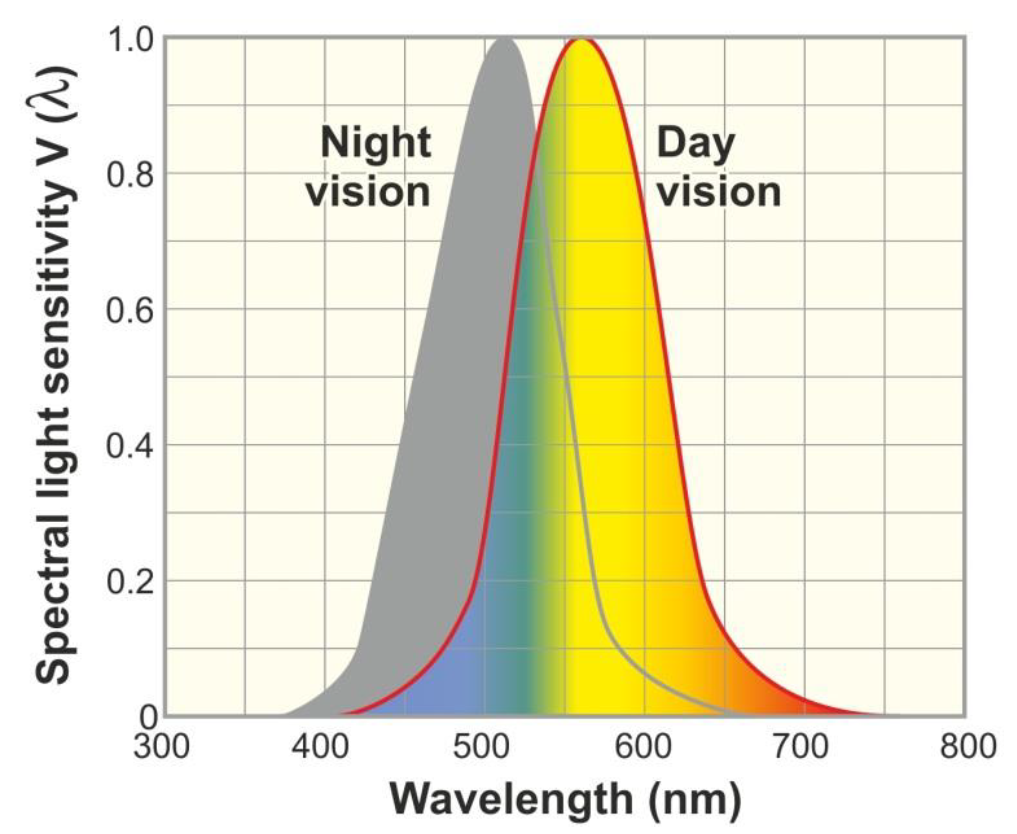
\includegraphics[width=0.4\linewidth]{vision}
\caption{Sensibilité de l'œil }
\label{vis}
\end{figure}

Pour obtenir la couleur d'un objet telle qu'elle sera perçu par l'œil humain, il suffit de multiplier le spectre de l'objet avec la courbe de sensibilité de l'œil.\\

La couleur de la source de lumière modifie aussi notre perception des couleurs. De manière analogue, il faut multiplier le spectre de la source avec la courbe de sensibilité de l'œil pour obtenir la couleur réellement perçue.





\newpage
\subsection{Caractéristiques optiques}
\subsubsection{Temperature de couleur}
Formellement, la température de couleur $[K]$ d'une source est la température à laquelle il faudrait chauffer un corps noir pour qu'il émette une lumière de même couleur que la source considérée.
La couleur apparente d'une source peut avoir des effets psychologique (ex : sensation d'inconfort) mais n'influence pas les performances visuelles.

\begin{figure}[h]
\centering
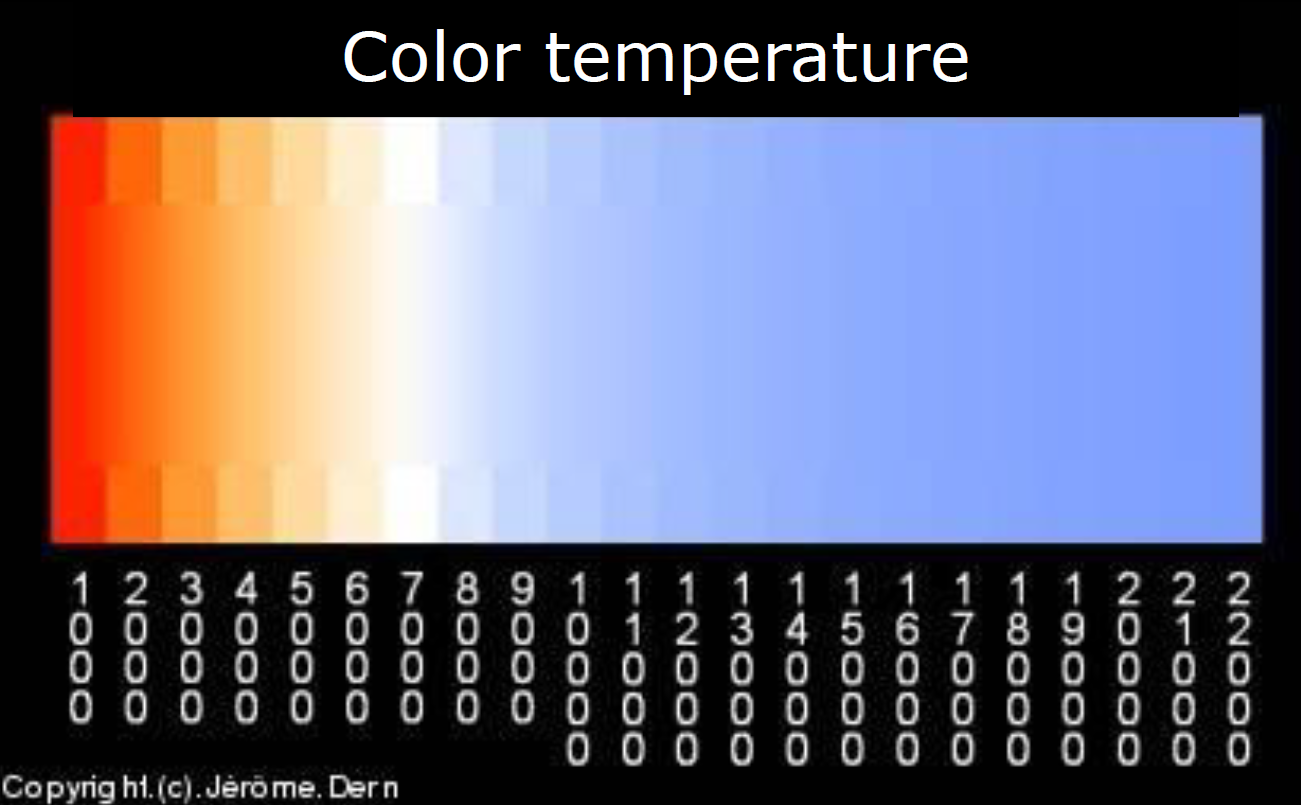
\includegraphics[width=0.4\linewidth]{temp}
\caption{Couleur de la lumière émise par une lampe en fonction de sa température}
%\label{vis}
\end{figure}


Le diagramme de Kruithoff donne les valeurs recommandées de température de couleur en fonction de la valeur de l'éclairement fournie par une lampe.


\begin{figure}[h]
\centering
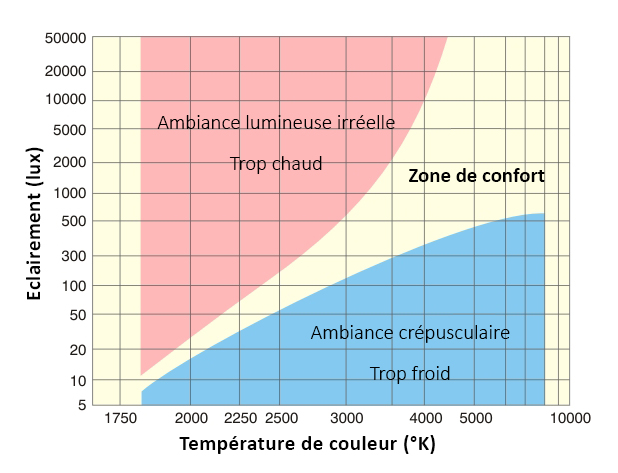
\includegraphics[width=0.4\linewidth]{krui}
\caption{Diagramme de Kruithoff}
%\label{vis}
\end{figure}

\subsubsection{Indice de rendu des couleurs, IRC}
\label{irc}
Une lumière sera d'autant plus qualifiée de "naturelle" que son spectre est continu. L'IRC noté $R_a$ quantifie cela. La lumière naturelle a un $R_a=100$. La norme EN 12464-1 donne la valeur minimale d'IRC en fonction du type de bâtiment, des locaux et des activités qui s'y déroulent. On peut aussi classer l'IRC en différentes classes.

\begin{center}
\begin{tabular}{cc}
\textbf{Classe de $R_a$} & \textbf{Valeur}\\
\hline
1A & $R_a > 90$\\
1B & $90 > R_a > 80$\\
2 & $80 > R_a > 60$\\
3 & $60 > R_a > 40$\\
\end{tabular}
\end{center}















%%%%%%%%%%%%%%%%%%%%%%%%%%%%%%%%%%%%%%%%%%%%%%%%%%%%%%%
\chapter{L'éclairage naturel}
\section{Composantes}
La lumière naturelle se décompose en 3 composantes.

\begin{minipage}{0.4\linewidth}
\centering
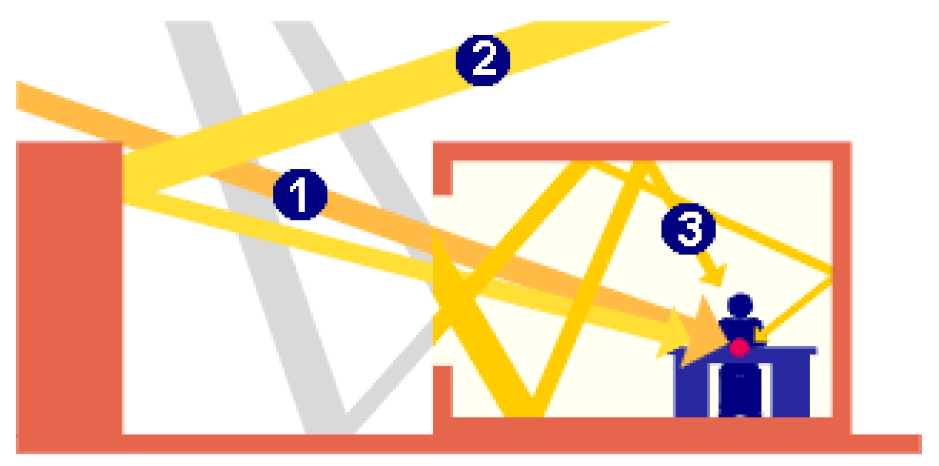
\includegraphics[scale=0.35]{compo}
\end{minipage}
\begin{minipage}{0.6\linewidth}
\begin{enumerate}
\item \textbf{Composante directe} qui dépend du climat, des ouvertures et des obstructions extérieures.
\item  \textbf{Composante réfléchie extérieure} qui dépend de la géométrie des surfaces extérieures de réflexion.
\item \textbf{Composante intra-réfléchie} qui est importante pour les locaux profonds.
\end{enumerate}
\end{minipage}


\vspace{5mm}
Pour optimiser l'éclairage d'un local, il est important d'optimiser les trois composantes selon les stratégies décrites ci-dessous.


\section{Stratégies}
%\begin{figure}[h]
%\centering
%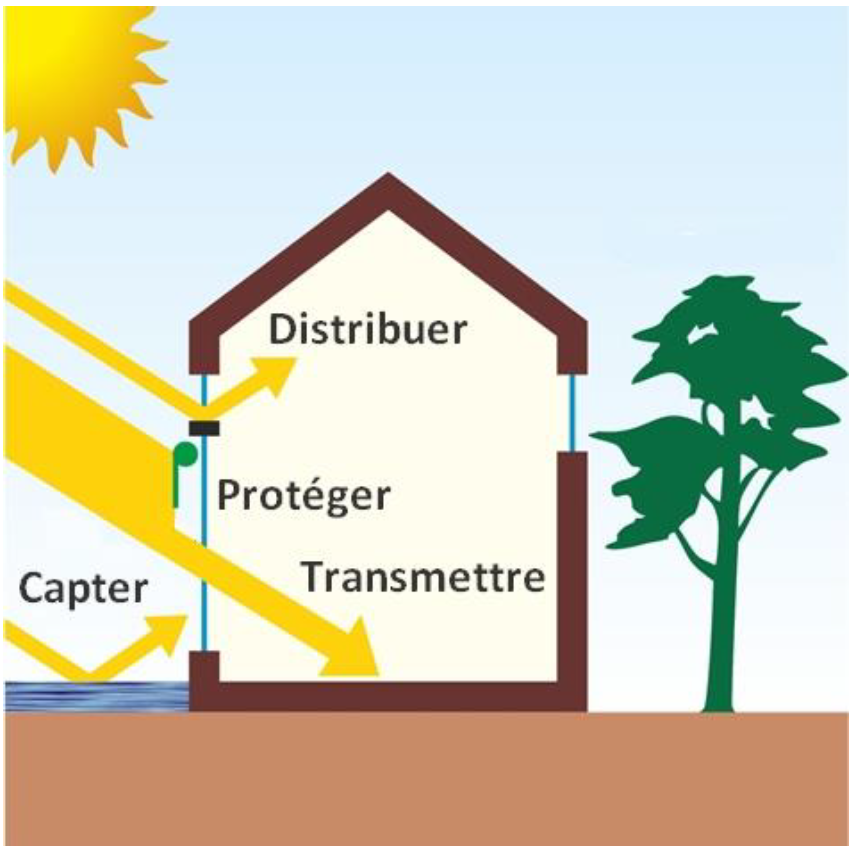
\includegraphics[scale=0.3]{strat}
%%\caption{Concepts pour optimiser}
%\end{figure}

\subsection{Capter}
\fcolorbox{white}{black!10}{\parbox{0.95\textwidth}{\begin{center} \textit{Consiste à collecter la lumière naturelle de manière à éclairer un bâtiment.}\end{center}}}\\


 La quantité de lumière à capter dépend de la localisation (latitude, altitude), du climat, du type de ciel, du moment de l'année, de l'heure, de l'orientation et inclinaison des ouvertures et de l'environnement physique (bâtiments voisins, type de sol, végétation).


\subsubsection{Position du soleil}
\begin{minipage}{0.7\linewidth}
La position du soleil dans le ciel est donné par sa hauteur $X \in [0^{\circ},90^{\circ}]$ et son azimut $Y\in [-90^{\circ},90^{\circ}]$ par rapport à l'axe sud. 
Il existe différents types de diagrammes qui permettent de représenter cela. Des diagrammes en coordonnées polaires ou cartésiennes.
\end{minipage}
\begin{minipage}{0.3\linewidth}
\centering
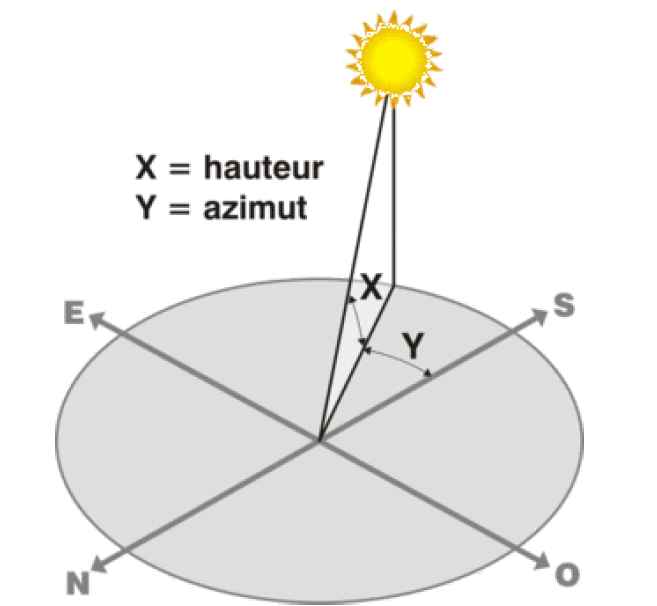
\includegraphics[scale=0.17]{az}
\end{minipage}


\vspace{5mm}
\begin{minipage}{0.5\linewidth}
\centering
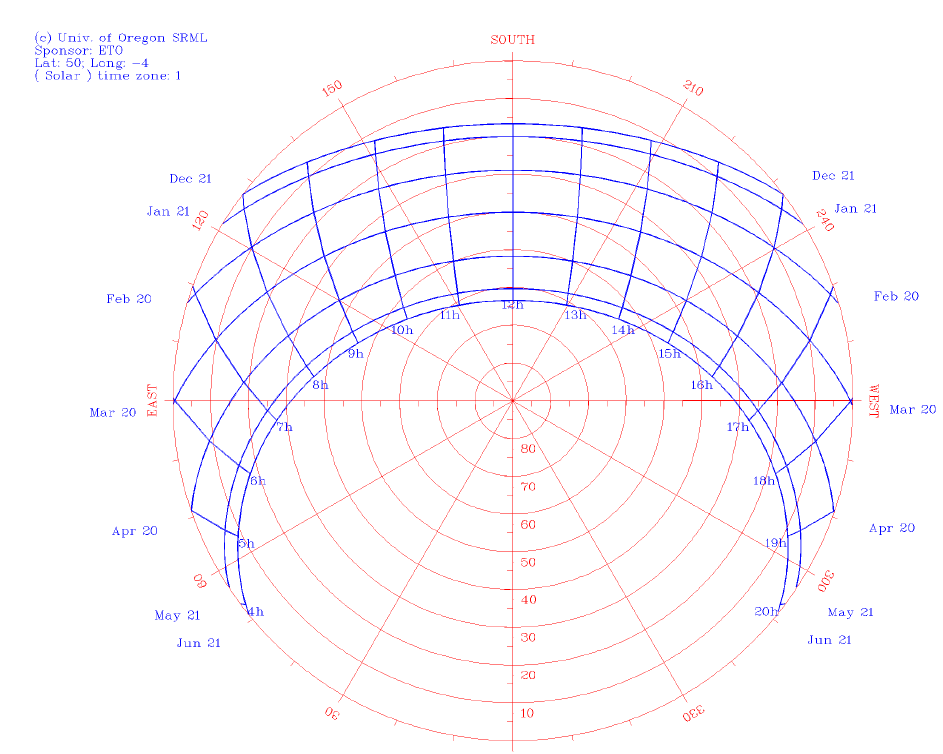
\includegraphics[width=0.65\linewidth]{pol}
\end{minipage}
\begin{minipage}{0.5\linewidth}
\centering
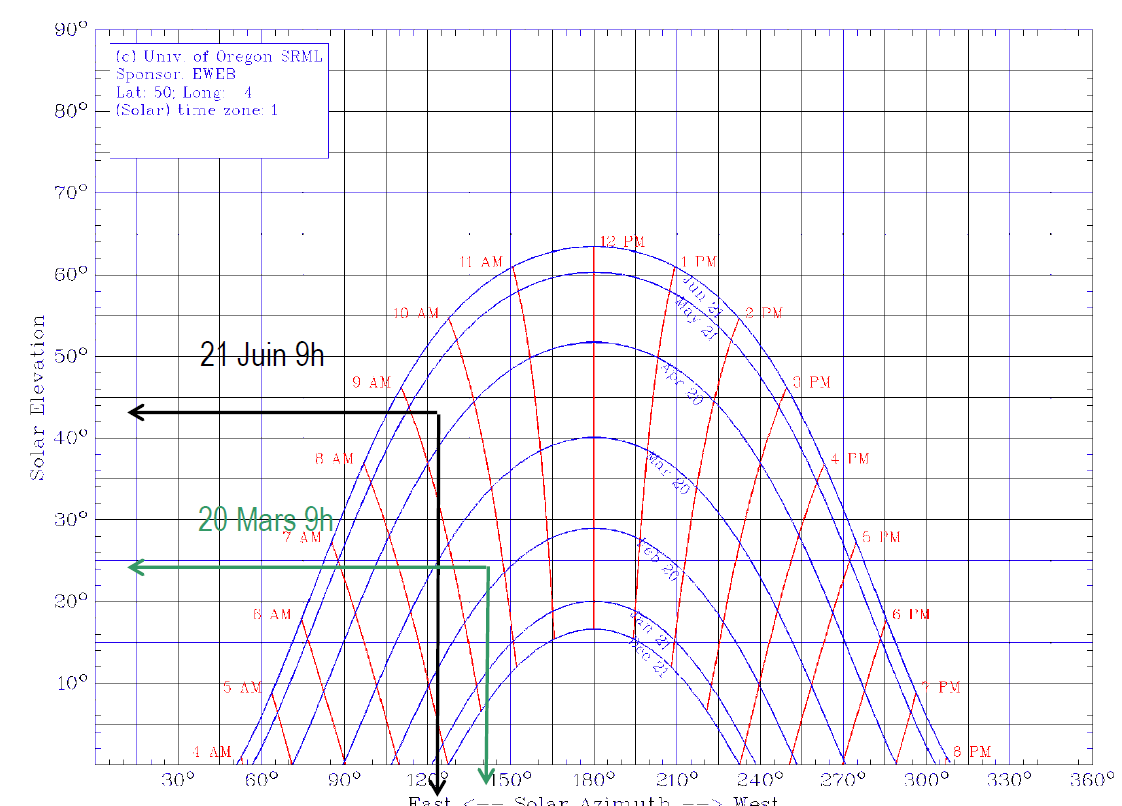
\includegraphics[width=0.65\linewidth]{cart}
\end{minipage}


\subsubsection{Type de ciel}
La lumière naturelle traduit les fluctuations de l'état du ciel. La composante directe dispense un flux considérable qui s'avère facile à capter et à diriger. C'est toutefois une source potentielle d'éblouissement et de surchauffe. De plus sa disponibilité est épisodique et dépends de l'orientation des ouvertures. La lumière diffuse ne présente pas ces risques mais est souvent largement insuffisante.\\


Vu la multitude de conditions météo existantes, des ciels standards ont été établis :\\


\underline{Ciel couvert :} Ce modèle correspond à un ciel de nuages clairs cachant le soleil. Sa luminance varie en fonction de la position du point de la voute céleste considéré suivant
$$L =L_z \frac{1+2 \sin \theta}{3}$$
où $L_z$ représente la luminance du zenith et $\theta$ la hauteur du point considéré. \\On voit donc que $L_z$ = $3 L_0$, la luminance de l'horizon.

\begin{figure}[h]
\centering
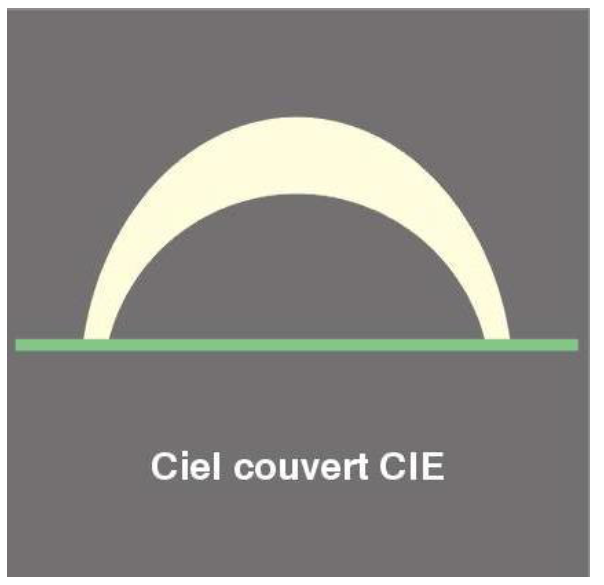
\includegraphics[scale=0.3]{couv}
\caption{Ciel couvert}
\label{cie}
\end{figure}




\subsubsection{Environnement Physique}
La lumière disponible dépend de l'environnement direct du bâtiment à travers le relief, les constructions voisines, le coefficient de réflexion du sol, la végétation, ...


On appelle \textit{masque solaire} tout corps empêchant le rayonnement solaire d'atteindre une surface que l'on désire ensoleillée.

\begin{figure}[h]
\centering
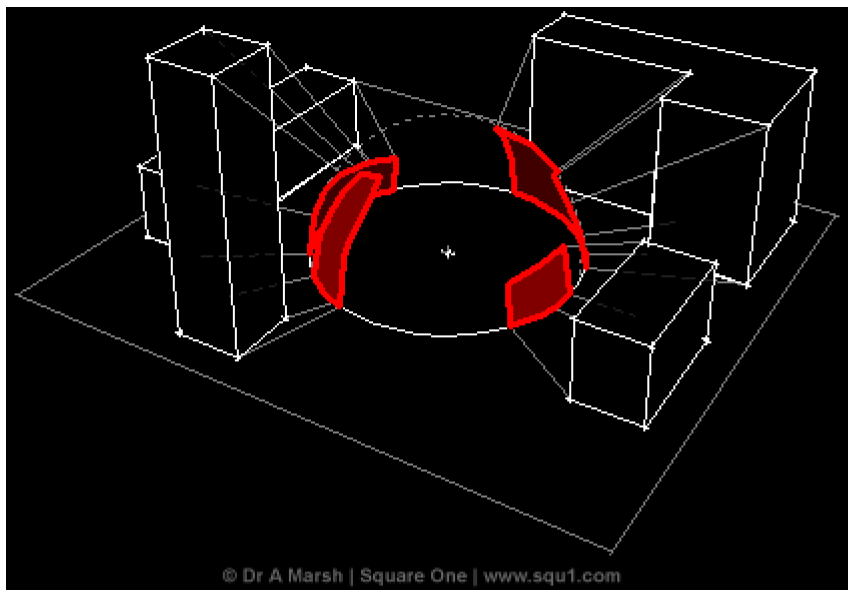
\includegraphics[scale=0.3]{masq}
%\caption{Ciel couvert}
\end{figure}


On tient compte de ce masque solaire pour dimensionner les ouvertures. Leur taille aura tendance à augmenter vers le bas des immeubles dans les ruelles étroites ou puits de lumières.\\


Le facteur de réflexion des surfaces extérieures n'est pas à négliger. La présence d'un lac par exemple, intensifie l'impression lumineuse d'un lieu mais peut également être une source d'éblouissement.





\subsubsection{Orientation des ouvertures}
\begin{center}
\begin{tabular}{llll}
\textbf{Orientation} & \textbf{Éclairement} & \textbf{Caractéristique} & \textbf{Divers}\\
\hline
Sud &  important & facile à contrôler & ensoleillement max en hiver\\
Est/Ouest & matin/soir & bas sur l'horizon & exposition faible en hiver\\
Nord & égal toute l'année & diffus & lumière homogène
\end{tabular}
\end{center}


\subsubsection{Inclinaison des ouvertures}
Par ciel couvert, la quantité de lumière arrivant en un point du local est proportionnelle à l'angle de vue du ciel. Pour une même superficie d'ouverture, cet angle sera toujours supérieur pour une ouverture zénithale que latérale. Et donc la lumière diffuse apportée aussi.

\begin{figure}[h]
\centering
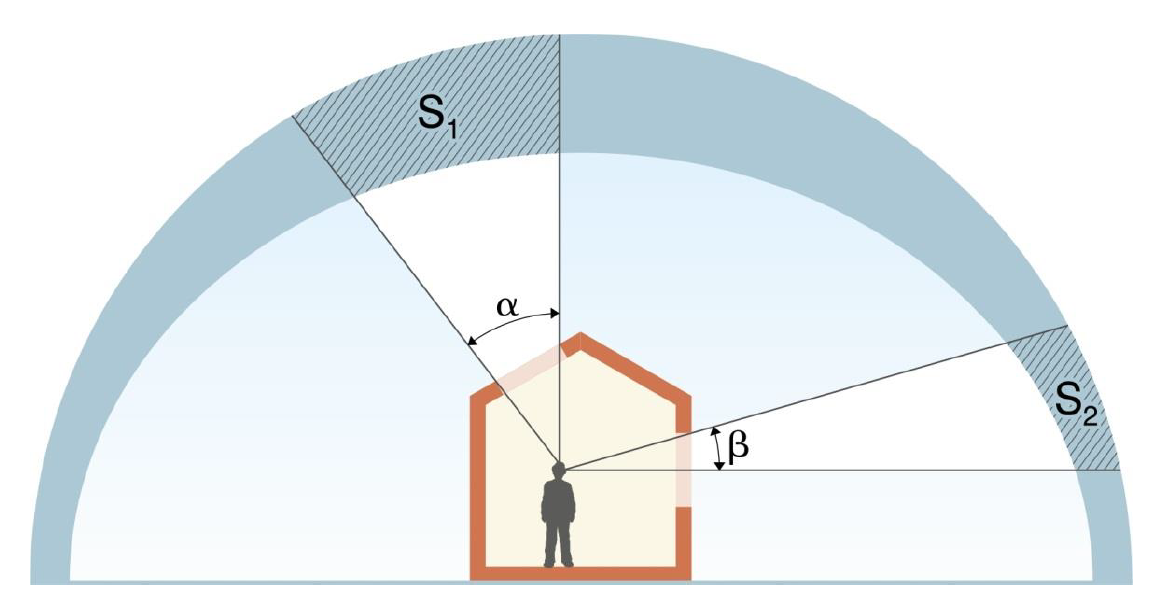
\includegraphics[scale=0.3]{zen}
%\caption{Ciel couvert}
\end{figure}


La Figure \ref{incl} est une simulation qui compare les deux solutions. La différence de clarté entre les deux locaux est frappante. Attention que les ouvertures zénithales sont souvent sources de gains solaire excessifs. Il faudra penser à s'en protéger (section \ref{protec}).

\begin{figure}[h]
\centering
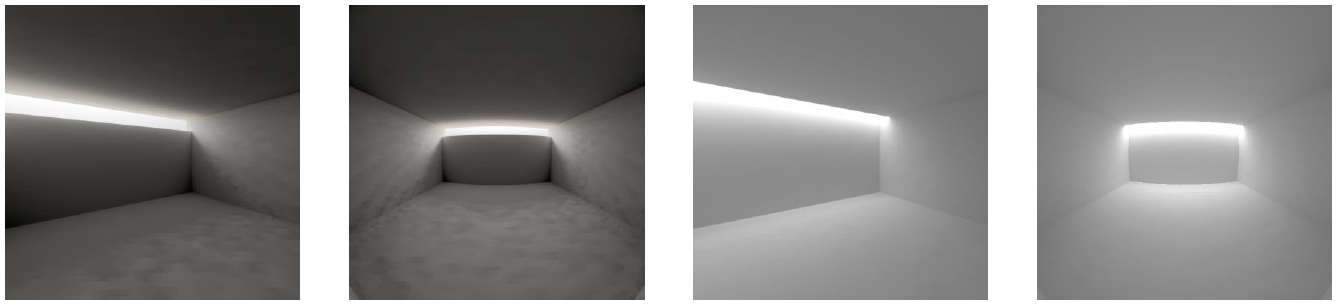
\includegraphics[width=\linewidth]{incl}
\caption{Ouverture latérale VS zénithale de même surface.}
\label{incl}
\end{figure}











\newpage
\subsection{Transmettre}
\fcolorbox{white}{black!10}{\parbox{0.95\textwidth}{\begin{center} \textit{Consiste à favoriser la pénétration de la lumière naturelle dans le bâtiment.}\end{center}}}\\

La quantité et qualité de lumière transmise dépend de la taille des ouvertures, leur forme, leur localisation et du matériau de transmission.

\subsubsection{Taille des ouvertures}
En reprenant la même simulation que ci-dessus et en faisant varier la surface des ouvertures :
\begin{figure}[h]
\centering
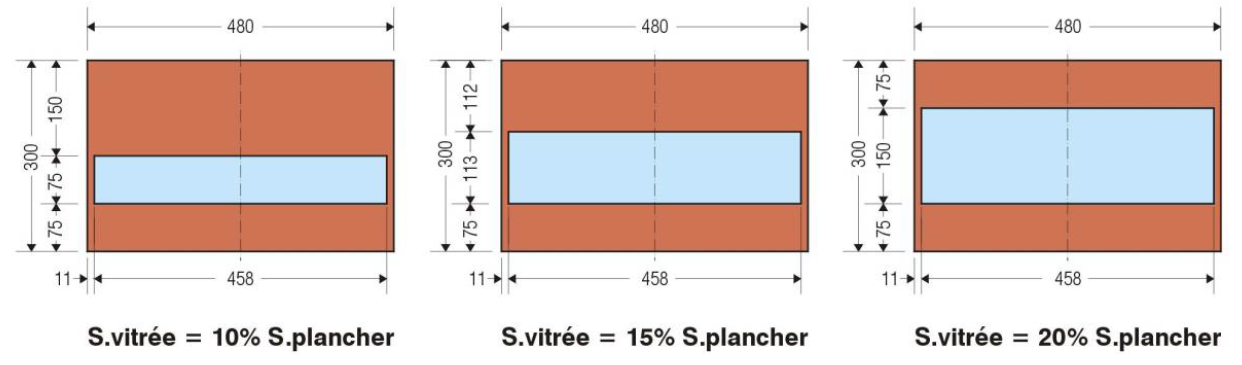
\includegraphics[width=0.6\linewidth]{svi}
\end{figure}

\begin{figure}[h]
\centering
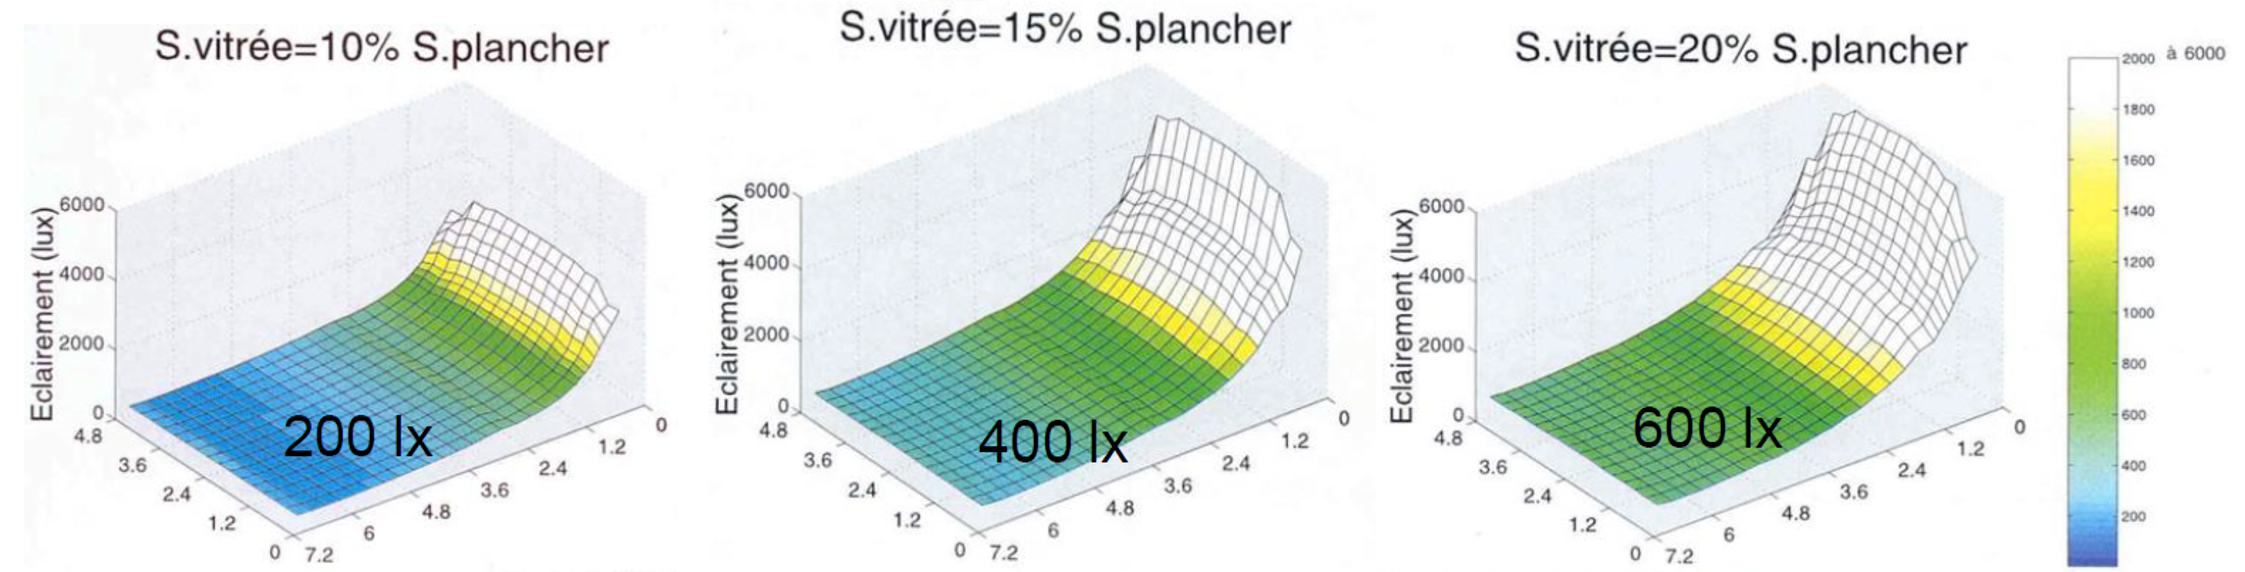
\includegraphics[width=\linewidth]{gra1}
%\caption{Ouverture latérale VS zénithale de même surface.}
\end{figure}

\begin{figure}[h]
\centering
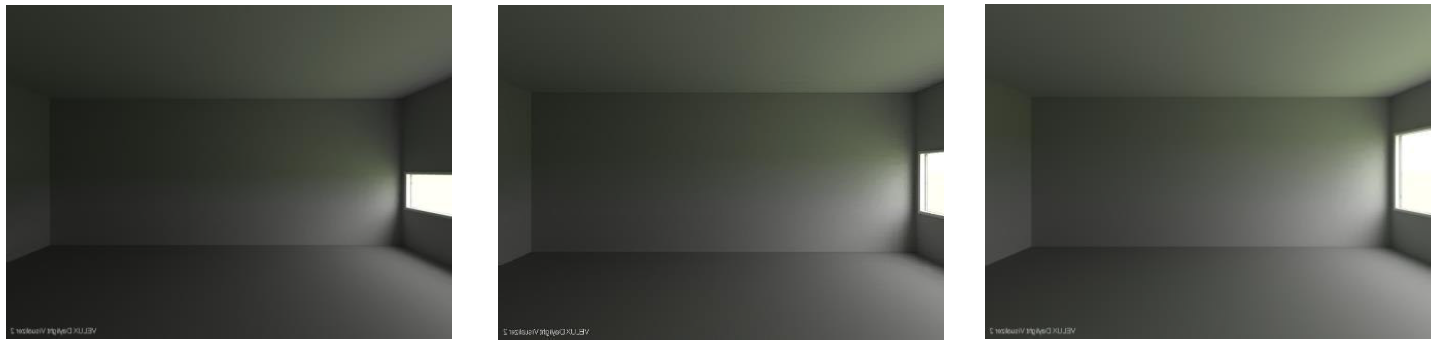
\includegraphics[width=\linewidth]{pho1}
%\caption{}
\end{figure}


\paragraph{Observations} On voit que c'est surtout l'éclairement en fond de local qui est affecté. Il augmente avec la taille de l'ouverture\footnote{C'est en fait plus la hauteur de la fenêtre qui produit ce résultat en fond de local, voir section sur la position.}. \\

Le chassis est aussi un élément important. Plus de surface de châssis veut dire moins de surface d'ouverture. La taille est fonction du type de fenêtre souhaité et du matériau :
$$\textup{bois} <\textup{ aluminium} < \textup{PVC}$$






\newpage
\subsubsection{Forme des ouvertures}
On fait varier la forme de l'ouverture cette fois : d'un rectangle très allongé à un carré avec la même surface et une hauteur d'allège constante.

\begin{figure}[h]
\centering
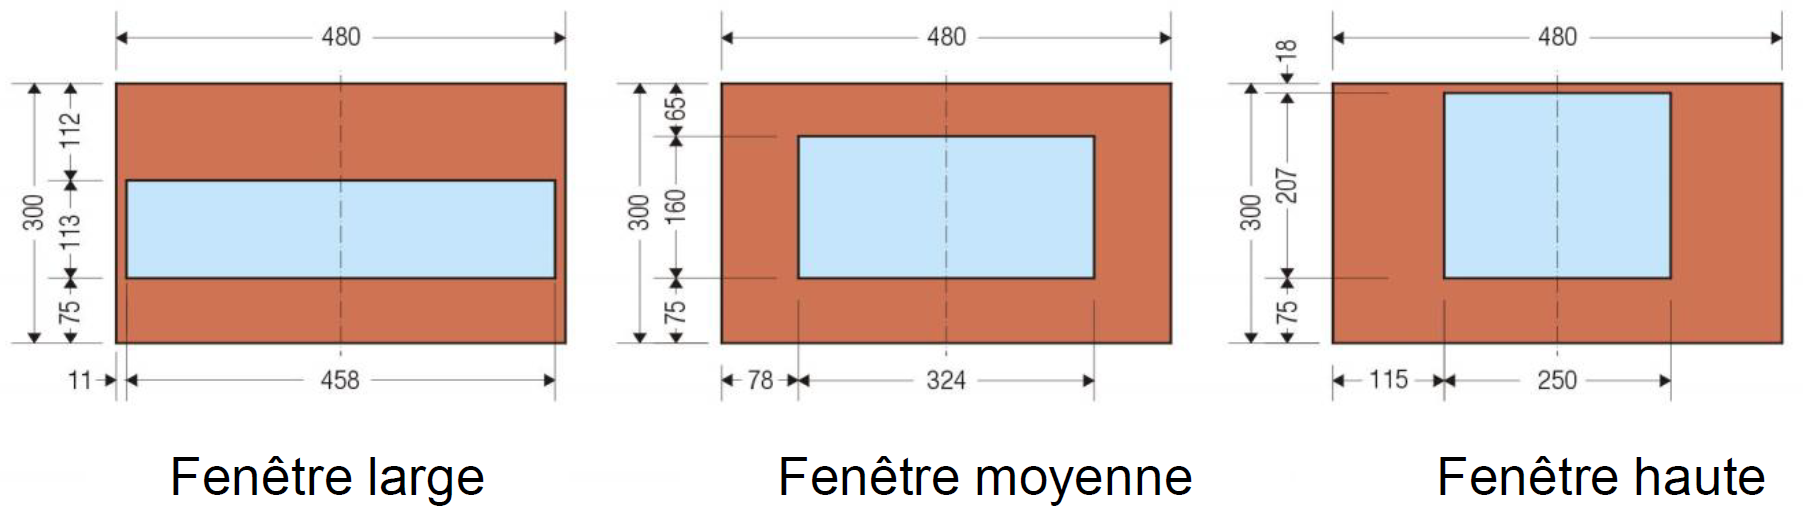
\includegraphics[width=0.6\linewidth]{forme}
\end{figure}

\begin{figure}[h]
\centering
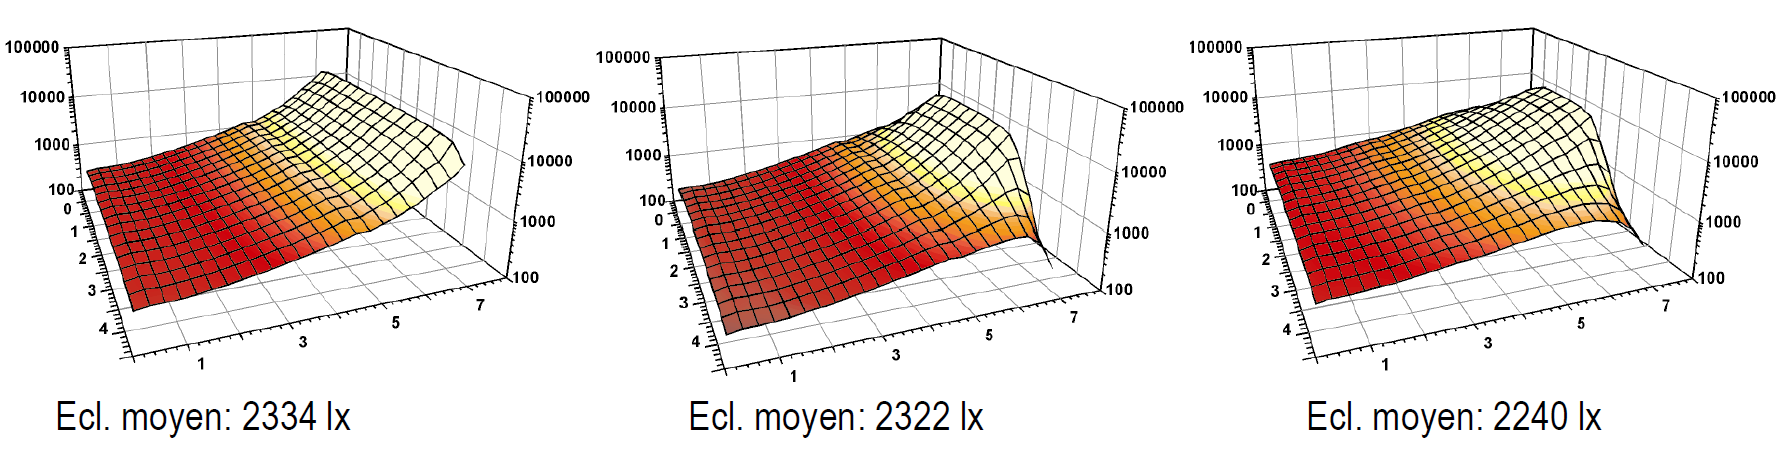
\includegraphics[width=\linewidth]{gra2}
%\caption{Ouverture latérale VS zénithale de même surface.}
\end{figure}

\begin{figure}[h]
\centering
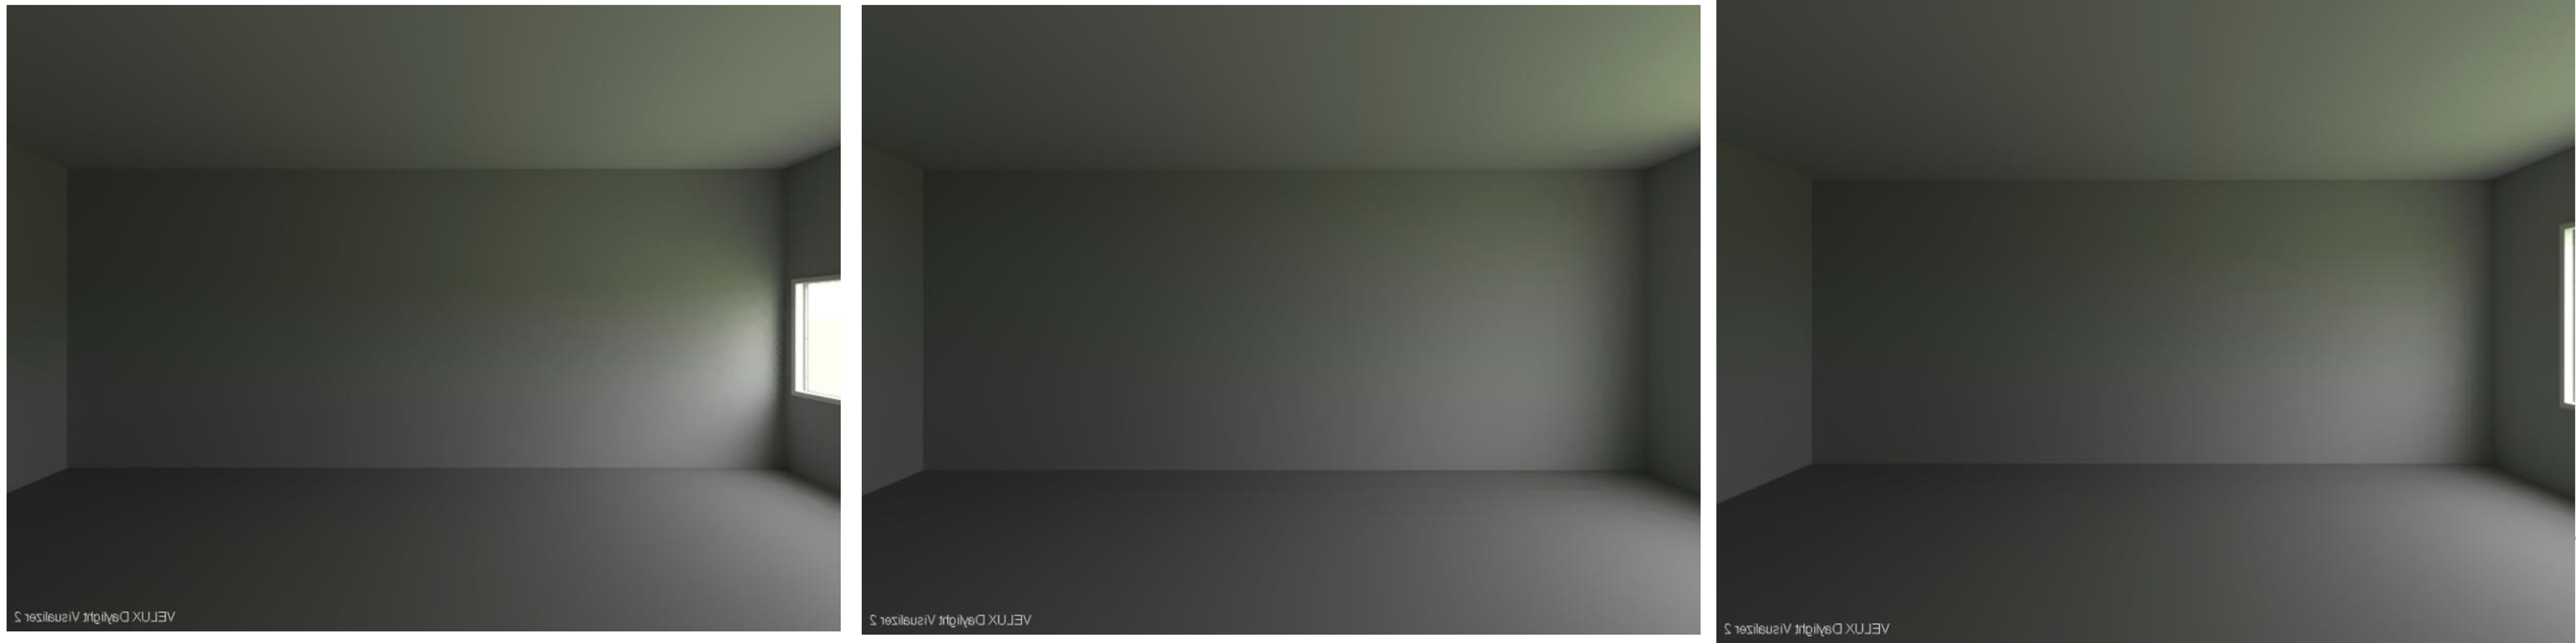
\includegraphics[width=\linewidth]{pho2}
%\caption{}
\end{figure}

\paragraph{Observations} On voit que l'on perd en uniformité d'éclairement autour de l'ouverture avec une fenêtre plus étroite mais qu'en moyenne on obtient les mêmes valeurs. L'étude du cas d'une seule fenêtre large ou de deux fenêtres étroites produit des résultats similaires.






\newpage
\subsubsection{Position des ouvertures}
On compare ici la hauteur de l'allège à surface constante.

\begin{figure}[h]
\centering
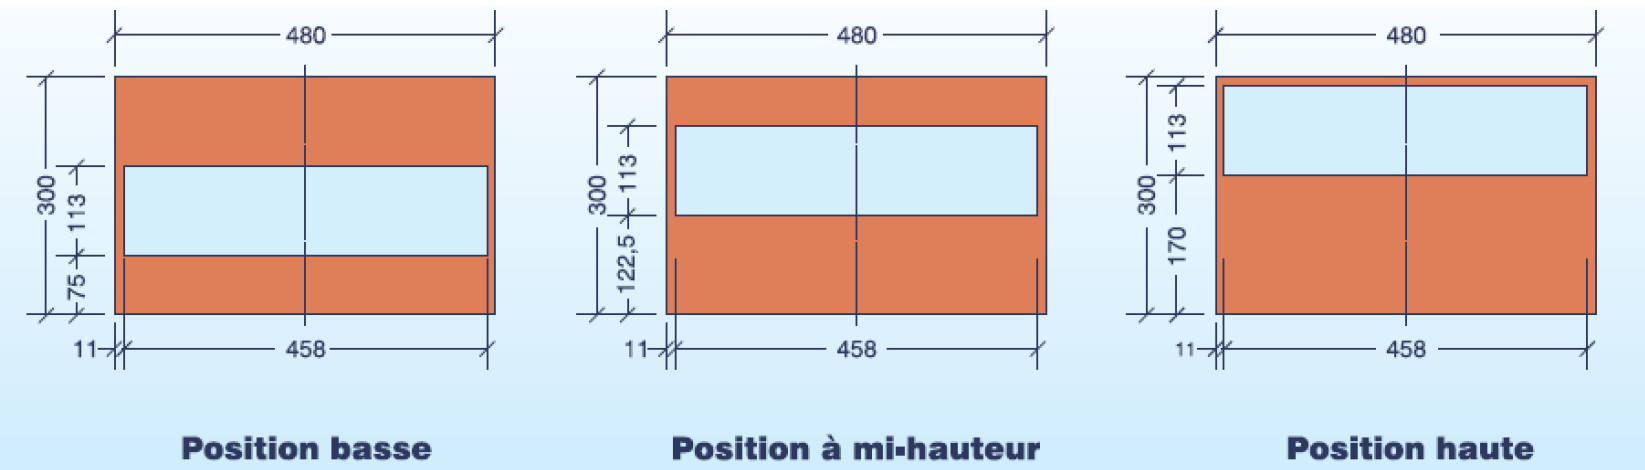
\includegraphics[width=0.6\linewidth]{hau}
\end{figure}

\begin{figure}[h]
\centering
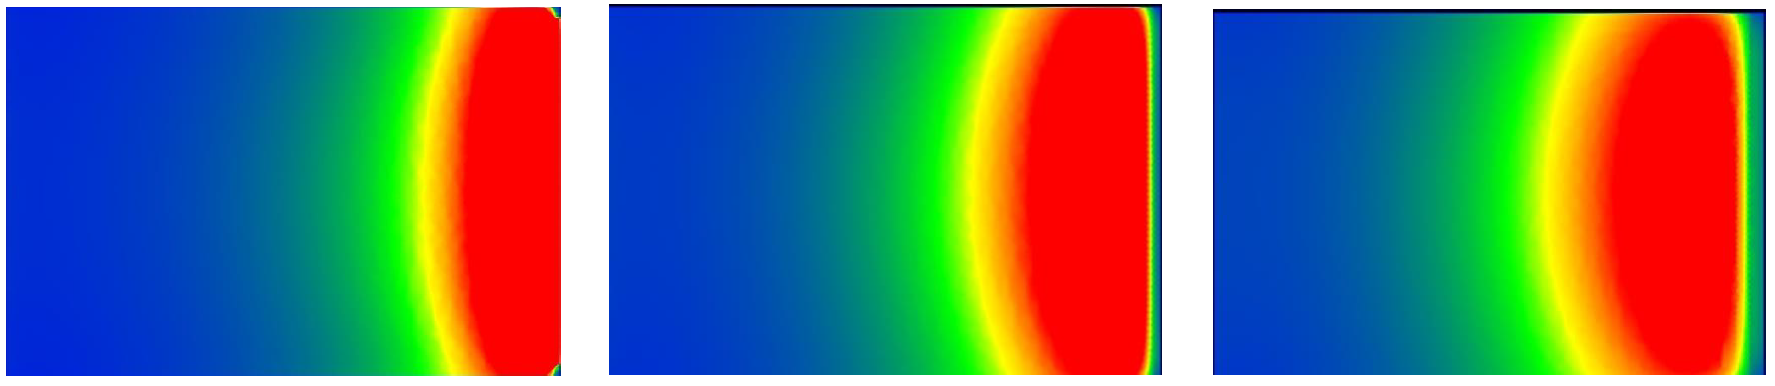
\includegraphics[width=\linewidth]{gra3}
%\caption{Ouverture latérale VS zénithale de même surface.}
\end{figure}

\begin{figure}[h]
\centering
\includegraphics[width=\linewidth]{pho3}
%\caption{}
\end{figure}


\paragraph{Observations} On voit que plus l'ouverture est élevée, mieux le fond du local est éclairé. On note aussi la création d'une zone d'ombre à proximité de la fenêtre d'autant plus importante que la fenêtre est haute.\\


Dans la plupart des cas, il est inutile de vitrer sous le niveau du plan de travail (gains solaires non souhaités) mais dans les bâtiments hauts, cela peut être souhaitable d'avoir une vue vers le bas.\\



\begin{minipage}{0.7\linewidth}
On appelle clerestory, toute fenêtre dont le seuil se trouve au dessus du niveau de l'œil. C'est pratique pour éclairer les fonds de locaux tout en limitant le risque d'éblouissement direct mais cela supprime la vue vers l'extérieur. On le couple donc souvent avec une autre fenêtre dotée d'une protection solaire. Exemple ci-contre à la bibliothèque d'Exeter de L. Khan.
\end{minipage}
\begin{minipage}{0.3\linewidth}
\centering
\includegraphics[scale=0.25]{bibli}
\end{minipage}




















\subsection{Distribuer}
\fcolorbox{white}{black!10}{\parbox{0.95\textwidth}{\begin{center} \textit{Consiste à diriger et à transporter les rayons lumineux de manière à créer une bonne répartition de lumière dans le bâtiment.}\end{center}}}\\


Une répartition harmonieuse de la lumière naturelle peut être favorisée par différentes approches basées sur le type de distribution, la répartition des ouvertures, l'agencement des parois intérieures et les matériaux des surfaces du local.



\subsubsection{Type de distribution}
Comme on l'a déjà dit, la lumière qui entre par voie directe constitue un flux important, créé un contact vers l'extérieur mais présente des risques d'éblouissement et de répartition très irrégulière dans un local.\\

L'éclairage naturel indirect utilise les réflexions sur diverses surfaces pour obtenir la distribution recherchée. Constitue une bonne protection contre l'éblouissement et produit une répartition homogène.
De plus une pièce ne possédant aucune fenêtre en contact direct avec l'extérieur peut être éclairée indirectement par des ouvertures donnant sur un ou plusieurs locaux éclairés directement. C'est ce qu'on appelle le second jour.

\begin{figure}[h]
\begin{minipage}{0.5\linewidth}
\centering
\includegraphics[width=0.9\linewidth]{kimbell}
\end{minipage}
\begin{minipage}{0.5\linewidth}
\centering
\includegraphics[width=0.9\linewidth]{jour}
\end{minipage}
\caption{Exemple d'éclairage indirect (gauche) et de second jour (droite)}
\end{figure}




\subsubsection{Répartition des ouvertures}
L'éclairage naturel provenant de plusieurs ouvertures peut s'évaluer approximativement en additionnant les éclairements issus des différentes sources. L'éclairage bilatéral produit un éclairage plus uniforme que l'éclairage unilatéral. Signalons que l'association d'un éclairage latéral et et zénithal est un cas particulier qui offre un très bon éclairage général et une mise en relief tridimensionnelle des objets. L'éclairage multilatéral est particulièrement indiqué dans les espaces nécessitant un éclairement très uniforme ainsi que dans les bâtiment profonds.

\begin{SCfigure}[20][h]
\centering
\includegraphics[width=0.5\linewidth]{multi}
\caption{Distribution lumineuse dans un local ouvert de manière latérale, bilatérale et multilatérale.}
\end{SCfigure}


\subsubsection{Agencement des parois intérieures}
Il faut veiller à ce que le mobilier ne constitue pas un obstacle à la pénétration de la lumière. Pour les locaux qui n'ont pas d'accès direct à une façade ou une toiture, l'utilisation de cloisons vitrées opaques ou transparentes (second jour) permettra de leur apporter un peu de lumière naturelle, toujours la bienvenue, même si elle doit être complémentée par de l'éclairage artificiel.



\subsubsection{Matériaux des cloisons et murs intérieurs}
La réflexion de la lumière sur les surfaces intérieures est généralement la composante principale de l'éclairement de fond de local.\\

Des parois de couleur claire assurent une répartition homogène de la lumière dans l'ensemble du local et sont bénéfiques au confort visuel en diminuant le contraste de luminance entre l'intérieur et l'extérieur.

Des parois sombres vont mal réfléchir et on va perdre en éclairement en fond de local tout en produisant une sensation visuelle d'obscurité. Rappelons en effet que l'œil évalue des luminances et non des éclairements. Entre une paroi blanche et noire de même éclairement, la paroi blanche paraîtra toujours plus lumineuse (Figure \ref{rh}). \\


\begin{figure}[h]
\centering
\includegraphics[width=\linewidth]{rho}
\caption{Ressenti visuel dans un local avec parois noires $\rightarrow$ blanches, sous les mêmes conditions d'éclairage}
\label{rh}
\end{figure}



On rappelle aussi que des surfaces mat vont parfaitement diffuser et produire un éclairage uniforme. Dans certains cas, il peut être intéressant de travailler avec des matériaux spéculaires pour renforcer la réflexion au fond du local. Attention aux risques d'éblouissement et à l'entretient de ces surfaces.\\

De manière générale : 
\begin{itemize}
\item si $\rho_{murs}<0,5$, la lumière pénétrera difficilement dans le local.
\item Le plafond qui est en général clair ne joue pas un rôle important.
\item Contrairement aux autres surfaces horizontales (sols, tables).
\end{itemize}





\subsection{Se protéger}
\label{protec}
\fcolorbox{white}{black!10}{\parbox{0.95\textwidth}{\begin{center} \textit{Consiste à arrêter partiellement ou totalement le rayonnement solaire lorsqu'il présente des caractéristiques néfastes à l'utilisation d'un local. Principalement l'éblouissement et ses aspects thermiques.}\end{center}}}\\

\subsubsection{Mobilité des protections solaires}
\begin{itemize}
\item \underline{Permanent :} Système fixe dont le degré de protection est constant (ex : films collés contre les vitrages).
\item \underline{Mobile :} Système pouvant être adapté en fonction de la position du soleil. Attention, leur emploi doit être efficace. Dans les bureaux paysagés, une fois que les stores sont baissés, on ne veut plus déranger les voisins et il est rare qu'on réouvre alors les stores. On ne profite plus du tout de la lumière naturelle.
\end{itemize}

\subsubsection{Limitation de l'éblouissement}
Il faut distinguer les causes de l'éblouissement pour pouvoir y remédier.
\begin{itemize}
\item \underline{Lumière directe:} Protections opaques
\item\underline{Lumière indirecte :} Vitres teintées, fins stores déroulables, rideaux clairs
\end{itemize}

\subsubsection{Diminution des surchauffes}
Bien placées, les protections peuvent supprimer la nécessité de climatisation ou du moins en limiter son utilisation et donc économiser de l'énergie. \\

Qu'elle soit à l'intérieur ou à l'extérieur, une protection solaire permet un contrôle sur la luminosité identique. Par contre, du point de vue thermique, il est toujours préférable de la placer dehors afin de prévenir le rayonnement d'entrer dans le bâtiment. Il y a alors des considérations esthétiques, d'encombrement de la façade, de résistance aux intempéries, d'entretient à prendre en compte.


\newpage
\subsubsection{Types de protection}
Il existe de nombreux types de protections solaires. \\

\begin{figure}[h]
\centering
\includegraphics[width=0.8\linewidth]{type}
\caption{Exemples de protections solaires classiques}
\end{figure}


La végétation peut aussi servir à réduire l'exposition d'une fenêtre au soleil. Les plantations doivent être choisies soigneusement en prenant en compte leur taille et leur type. 

\begin{figure}[h]
\centering
\includegraphics[width=0.6\linewidth]{arbre}
\caption{Protection solaire végétale}
\end{figure}




























\newpage
\section{Les métriques en éclairage naturel}
\subsection{Facteur de lumière du jour}
\begin{minipage}{0.4\linewidth}
\centering
\includegraphics[scale=0.35]{flj}
\end{minipage}
\begin{minipage}{0.6\linewidth}
Le FLJ est défini comme le rapport de l'éclairement naturel reçu en un point (plan de travail) sur la valeur de l'éclairement horizontal d'un point extérieur situé en un site parfaitement dégagé (toit du bâtiment). Le type de ciel utilisé est le ciel couvert.
$$FLJ(i) = \frac{E(i)}{E_0}.100 \;\;\;\;\;\;\;\;\;[\%]$$

Le FLJ fournit une quantité mesurée et standardisée qui permet la comparaison de différents bâtiments.
\end{minipage}

\vspace{1cm}
Un bâtiment ne doit pas être dimensionné sur base du FLJ car puisque c'est une mesure standardisée, elle ne prend pas en compte un certain nombre de facteurs.
\begin{itemize}



\item \textbf{Orientation}
Le FLJ est calculé sous un type de ciel couvert (Figure \ref{cie}) dont la luminance ne varie pas en fonction de l'orientation. Or une façade orienté au Nord ou au Sud ne recevra pas la même lumière. 
\item \textbf{Valeurs maximales}
Les valeurs de FLJ recommandées par les normes sont en général des valeurs minimales. Le fait de respecter ces normes ne signifie pas que le bâtiment ne sera pas survitré ce qui peut amener à des problèmes thermiques et d'éblouissement. Les occupants vont alors mettre en place des systèmes de protection avec le risque de stopper complètement toute pénétration de la lumière naturelle et d'induire des surconsommations d'éclairage électrique. 
\item \textbf{Latitude}
\item \textbf{Climat}
\end{itemize}

\begin{figure}[h]
\centering
\includegraphics[scale=0.5]{flj1}
\caption{FLJ pour un local avec et sans ouverture zénithale}
\end{figure}


\newpage
\subsection{Autonomie dynamique}
C'est le pourcentage des heures d'occupation d'un local durant lesquelles le niveau minimum d'éclairement requis peut être assuré par la lumière naturelle seule.

\begin{figure}[h]
\centering
\includegraphics[scale=0.5]{bos}
\caption{Exemple de carte temporelle}
\end{figure}



\subsection{Éblouissement}
Le Daylight Glare Probability (DGP) est une approche qui considère l'éclairement au niveau de l'œil ainsi que les $n$ sources individuelles d'éblouissement potentiel de manière à estimer la fraction de personnes insatisfaites par les conditions lumineuses. Le DGP est défini par une formule empirique qui fait intervenir des grandeurs photométriques 

$$DGP = c_1 E_v + c_2 \log \Bigg( 1 + \sum_i^n \frac{L^2_{s,i} \omega_{s,i}}{E_v^{c_4} P^2_i}\Bigg) + c_3$$
 
 avec $E_v$ l'éclairement vertical au niveau de l'œil, $L_s$  la luminance des sources d'éblouissement, $\omega_s$ l'angle solide sous-tendu par chaque source et $P$ l'indice de Guth. \\
 
 Les valeurs de DGP peuvent être catégorisée de la manière suivante :
 
 \begin{center}
 \begin{tabular}{lc}
 \textbf{Eblouissement}&\\
 Imperceptible & $DGP < 0,35$\\
 Perceptible & $0,35 < DGP < 0,40$\\
 Dérangeant & $0,40 < DGP < 0,45$\\
 Intolérable & $0,45 < DGP$\\
 \end{tabular}
 \end{center}


\chapter{Annexes}
\section{Courbes de répartition photométriques}
\label{an1}
Voici quelques exemples complémentaires de diagrammes polaires de répartitions d'intensité lumineuse. L'intensité lumineuse $[cd]$ est représentée par les différents cercles sur le schéma. Plus le cercle est grand, plus la valeur en candela est élevée.

Pour les luminaires symétriques, les courbes se superposent.

\begin{figure}[h]
\centering
\includegraphics[width=\linewidth]{luminaires}
\caption{Exemple de luminaires de chez DMLights}
\end{figure}


%\section{Sources}
%\begin{itemize}
%\item Syllabus et slides du cours [LICAR1821] de Magali Bodart
%\item "Comment interpréter une courbe de répartition photométrique?" par DMLights consulté le 06 janvier 2018\\
%\textit{https://www.dmlights.fr/blog/comment-interpreter-une-courbe-de-repartition-photometrique/}
%\end{itemize}




\part{Acoustique}
\chapter{Caractérisation du bruit et des équipements}
\section{Généralités}
\paragraph{Définition} Une onde acoustique est une vibration de l'air due à une suite de pressions/dépressions.

Ces ondes nécessitent un milieu pour se propager. La vitesse du son dans un milieu est fonction de la température $T\,[K]$
$$v_{son} = 20 \sqrt{T} = 340 \;m/s\hspace{1cm} \textup{dans l'air à 16}^{\circ}C$$
On notera que l'air est un milieu non dispersif c'est à dire que toutes les fréquences arrivent en même temps.

\section{Intensité}
L'intensité d'un bruit est l'impression de force sonore qu'il exerce sur l'oreille. On peut l'interpréter différemment dans deux domaines.

\paragraph{Physique} On considère l'intensité comme un flux d'énergie par unité de temps et de surface $I\;[W/m^2]$.

\paragraph{Physiologique} On considère un niveau d'intensité acoustique $L_p\;[dB]$.
$$L_p = 10 \log \frac{I}{I_0} = 10 \log \frac{p^2}{p^2_0} = 20 \log \frac{p}{p_0} $$

\fcolorbox{white}{black!10}{\parbox{0.95\textwidth}{
\begin{center}
\begin{tabular}{rl}
\multicolumn{2}{c}{\textbf{Échelle des niveaux de pression $[dB]$}}\\
$120$ & Seuil de douleur\\
$100$ & Musique amplifiée à risque\\
$80$ & Seuil d'exposition limitée dans le temps\\
$70$ & Circulation moyennement dense\\
$60$ & Conversation\\
$40$ & Extérieur, lotissement calme\\
$30$ & Intérieur, chambre calme\\
$20$ & Intérieur excessivement calme\\
$0 $ & Seuil de l'audition humaine\\

\end{tabular}
\end{center}
}}\\

\section{Hauteur}
\label{high}
La hauteur d'un bruit est définie par sa fréquence $f\;[Hz]$ avec 
$$\lambda = \frac{v}{f}$$
L'oreille humaine est limitée à un spectre de fréquences audibles :
$$\textup{Infrasons} < 20 \,Hz < f < 15 \,kHz < \textup{Ultrasons}$$

Il est très difficile de se protéger des infrasons (transports, métro, ...) car ces ondes ont des $\lambda$ de plusieurs mètres. Au contraire, on arrête facilement les ultrasons avec quelques $cm$ d'isolant. Typiquement, un bruit de voix est à $500\,Hz$.\\

On différencie les sons, qui ont un spectre périodique (fondamentale et harmoniques), aux bruits, qui ont un spectre aléatoire.



\subsection{Phénomène}
\subsubsection{En phase}
\subsubsection{En opposition de phase}
\subsubsection{Stationnaire}


\subsection{Intervalle de fréquence}
\paragraph{Définition }

\paragraph{Exemple }







\section{Pondération A}
\paragraph{Définition } Le $dB(A)$ est une mesure de la sensation réelle (physiologique). En effet, l'oreille n'entend pas avec la même force deux sons de $f$ différentes qui ont la même intensité (physique). \\

Il existe d'autres types de pondération: ...

...
$$L_{A,eq,T} = 10 \log \Bigg ( \frac{1}{t_2-t_1} \int_{t_1}^{t_2} \frac{p_A^2(t)}{p^2_0}dt \Bigg)$$



ordres de grandeurs...


...

\section{Sonomètre}
...


\section{Bruit de fond}
emergence..

$$E=L_{AS,max,T}-L_{A,eq,T}$$


tableau avec normes



\section{Addition des niveaux sonores}
Puisqu'on travaille en $dB$, on ne peut pas simplement additionner les niveau comme ça. On utilise la \textit{règle de sommation des niveaux}:
$$L_p = 10\log \Big( 10^{\frac{L_{p1}}{10}}+10^{\frac{L_{p2}}{10}}+...+10^{\frac{L_{pn}}{10}} \Big)$$

On note qu'a partir d'une différence de $\Delta=10\,dB$ entre deux sources, la plus grande masque totalement la plus faible.


\paragraph{Exemple } L'addition d'une source à $70\,dB$ et une à $60\,dB$ donne
$$L_p = 10\log \Big( 10^{\frac{70}{10}}+10^{\frac{60}{10}}\Big)=70,4 \simeq 70 \,dB$$


\section{Puissance acoustique}
...
\paragraph{Source ponctuelle} Source considérée petite comparée à la distance qui la sépare du récepteur, assimilable à un point. Propagation sphérique.
$$L_p=L_w-20 \log d - 8$$

Le niveau de pression acoustique diminue de $6\,dB$ par doublement de la distance.

\paragraph{Source linéaire} Source allongée, assimilable à une ligne. Propagation cylindrique.
$$L_p=L_w-10 \log d - 5$$

Le niveau de pression acoustique diminue de $3\,dB$ par doublement de la distance.




\section{Bruits des installations techniques}
...
A la conception, pour éviter un maximum les bruits des installations techniques, on construit chambre contre chambre, etc...\\

La présence des techniques (évacuations sanitaires, ventilation, hottes, ascenseurs, ...) dans les parois acoustiques sont des risques de déforcement.\\

\subsection{Évacuation sanitaires}
On essaye un maximum de désolidariser de la structure les appareils et les conduites. Dans les immeubles à appartements:

\subsubsection{Directives pour les conduites d'évacuations}
\begin{itemize}
\item Toujours en gaine, pas d'encastrement
\item Fixations munies de colliers antivibratiles\footnote{\#Nouveaux urinoirs du Sciences}
\item Fixation sur la paroi la plus lourde
\item Conduites en PE plutôt qu'en PVC($-5\,dB$)
\item Passage désolidarisé au droit des planchers
\end{itemize}

\subsubsection{Directives pour la fermeture des gaines techniques}
\begin{itemize}
\item Laine minérale sur $50\%$ des parois intérieures
\item Blocs de plâtres de $10\,cm$ si locaux peu sensibles
\item Double épaisseur $7+10\,cm$ ou paroi lourde si locaux sensibles.
\item Double structure métallique possible avec 2x2 plaques de plâtres + laine minérale\footnote{Effet masse-ressort-masse, section \ref{MRM}}
\end{itemize}



\subsection{Ventilation}
Dans les immeubles à appartements, on préfère l'utilisation de groupes individuels qui sont plus facile à gérer. Ces groupes font du bruit aussi bien à la pulsion qu'à l'extraction d'air mais on a aussi des risques secondaires tels que de l'interphonie via le réseau, des nuisances acoustiques vers l'environnement, des fuites, ...\\

Le choix du groupe en lui-même est déterminant sur le niveau de bruit. On sélectionne un ventilateur pour $75\%$ de sa puissance max requise.\\

\subsubsection{Directives pour les groupes de ventilation}
\begin{itemize}
\item Fixation sur la paroi/plancher le plus lourd
\item Éloigné de tout locaux sensibles
\item Éviter tout contact rigide avec la structure 
\item Appuis/suspentes antivibrtiles
\end{itemize}


Le réseau doit être configurer pour limiter les pertes de charges et donc les turbulences car le bruit est proportionnel à la vitesse de l'air.


\subsubsection{Directives pour le réseau de ventilation}
\begin{itemize}
\item Sections suffisamment larges en fonction du débit
\item Éviter les conduites souples (longueur limitée, tracé droit)
\item Parois des conduites lisses, on limite le nombre de raccords
\item Coudes courbés, rayon de courbure $>$ diamètre de la conduite
\end{itemize}


On peut aussi utiliser des silencieux. Ils sont à placer avant la sortie du local technique, près du groupe. Ce qui est un bon compromis entre pertes de charges, atténuation et encombrement. On notera que si la vitesse dans les conduites dépasse $5\,m/s$, le bruit du ventilateur domine le bruit de flux.\\


\subsubsection{Directives pour la traversée de parois massives}
\begin{itemize}
\item Ouverture au plus près de la conduite
\item Aucun contact conduite/structure
\item Membrane souple autour de la conduite
\item Laine minérale ou mousse acoustique
\item Cimentage/enduit
\end{itemize}


Comme partout ailleurs en acoustique, on veillera à une \textbf{parfaite étanchéité} puisque c'est l'élément le plus faible qui détermine l'isolation de toute la paroi.

\subsection{Ascenseurs}
Pour les cages d'ascenseurs, on utilise des doubles structures lourdes ou des structures lourdes avec doublage.



\chapter{Correction acoustique des salles}
\section{Coefficient d'absorption}

Pour commencer il est important de différencier isolation et absorption acoustique (Figure \ref{ene}).


\begin{center}
\begin{tabular}{cc}
\textbf{Isolation} & \textbf{Absorption}\\
$\frac{E_i}{E_t}\;[dB]$ & $\frac{E_i}{E_r}\;[-]$
\end{tabular}
\end{center}
energies ou puissances??


\begin{figure}[ht]
\centering
\includegraphics[width=0.5\linewidth]{ene}
\caption{Isolation VS absorption acoustique}
\label{ene}
\end{figure}

\paragraph{Exemple :} le chanvre est un très bon absorbant (0,65) mais est peu isolant (5 dB) alors qu'un panneau de bois sera peu absorbant (0,2) mais possède une capacité d'isolation intéressante (29 dB).\\


On définit le \textit{coefficient d'absorption acoustique} $\alpha\;[-]$ 
$$\alpha = \frac{W_a+W_t}{W_i} = 1 - \frac{W_r}{W_i}$$

avec $W_i = W_r + W_a + W_t$. Une valeur d'$\alpha=0$ indique de tout est réfléchi et $\alpha=1$ indique de rien est réfléchi c'est à dire que tout est transmis et/ou absorbé. C'est fonction de la fréquence et de l'angle d'incidence.
\\

\subsection{En champ libre} Le niveau de puissance et le niveau de pression à une distance $d$ sont reliés par
$$L_p = L_w + 10 \log \frac{Q}{4\pi d^2} = L_w - 20 \log d - 8 \hspace{1cm} $$
La dernière égalité est obtenue pour un \textit{facteur de directivité} $Q=2\,[-]$. 
\subsection{En espace clos} La relation ci-dessus n'est pas valable car l'énergie sonore réfléchie par les parois $I_r$ s'ajoute à l'énergie directement rayonnée par la source $I_d$
$$I = I_d + I_r = \frac{W}{4 \pi d^2} + 4W \frac{1-\alpha_{moy}}{S \alpha_{moy}}$$

avec $W$ la puissance de la source et $S$ la surface totales des parois du local. Le terme $\alpha_{moy}$ est défini comme
$$\alpha_{moy} S = \sum \alpha_i S_i + \sum A_j$$
où $\alpha_i$ est le facteur d'absorption du matériau $i$, $S_i$ sa surface et $A_j$ l'aire d'absorption équivalente pour l'objet $j$. On peut aussi écrire 
$$I = I_d + I_r = \frac{W}{4\pi d^2}\Bigg( 1 + \frac{16\pi d^2}{R} \Bigg)$$

On a introduit la \textit{constante d'absorption du local} $R\,[m^2]$ telle que 
$$R = \frac{S \alpha_{moy}}{1-\alpha_{moy}}$$


Il est intéressant de connaître pour un local la distance $d_0\,[m]$ appelée \textit{distance critique} pour laquelle $I_d = I_r$
$$d_0 = \sqrt{\frac{R}{16 \pi}}$$

Dans une habitation, pour une pièce normalement meublée, $0,75\,m < d_0 < 1\,m$.

La relation finale entre le niveau de puissance et le niveau de pression en espace clos est
$$L_p = L_W+ 10 \log \Bigg( \frac{Q}{4 \pi d^2} + \frac{4}{R} \Bigg)$$

On observe une diminution de $3\,dB$ lorsqu'on double la quantité d'absorbant ($2A$)\footnote{A et R sont la même chose...}.


\section{Temps de réverbération}
\paragraph{Définition } Le temps de réverbération $T\,[s]$ est le temps nécessaire à une diminution de $60\,dB$ lors de l'interruption nette d'un bruit.\\

$T$ augmente avec $V\,[m^3]$ le volume du local et diminue avec la quantité d'absorption dans le local $A\,[m^2]$. On dispose de plusieurs moyen de le calculer. 
\begin{center}
\begin{tabular}{lc}
\textbf{Formule d'Eyring :} & $T=\displaystyle\frac{0,16 V}{4 m V- S \ln (1-\alpha_{moy})}$\\
&\\
\textbf{Formule de Sabine :} & $T=\displaystyle\frac{0,16 V}{4mV + A}$\\
\end{tabular}
\end{center}
avec $m$ le coefficient d'atténuation lié au milieu (air).


Dans la pratique, nous utilisons la formule de Sabine simplifiée 

\fcolorbox{white}{black!10}{\parbox{0.95\textwidth}{$$T=\displaystyle\frac{0,16 V}{A}$$}}\\

qui permet une rapide estimation à condition que la répartition des absorbant soit homogène. Cette formule est d'autant moins valide que la salle est absorbante (inutilisable pour $\alpha_{moy}>2$, surestimation de $T$).\\

En acoustique, on manipule souvent la moyenne pondérée pour tout le spectre de fréquence d'une grandeur. On la dénote par un indice $_w$ pour "weighted". Ainsi, on utilise $\alpha_w$ comme valeur représentante de $\alpha$ à toutes les fréquences. 

\section{Ordres de grandeur et Exigences}
\fcolorbox{white}{black!10}{\parbox{0.95\textwidth}{

\begin{center}
\begin{tabular}{|lrc|clr|}
\hline
\multicolumn{2}{|c}{\textbf{Temps de réverbération}} &&& \multicolumn{2}{c|}{\textbf{Coefficient d'absorption}}\\
\textbf{Type de Local} & $T\,[s]$ &&& \textbf{Matériau} & $\alpha_w$\\
\hline
Bureau individuel & 0,6 - 0,8 &&& Vitre & 0,05 \\
Bureaux paysagés &&&& Béton non peint & 0 \\
\hspace{10mm}$<200 \, m^2$ & 0,6 - 0,8 &&& Plâtre & 0,05 \\
\hspace{10mm}$<200 \, m^2$ & 0,8 - 1,0 &&& Bois vernis & 0,05 \\
Salle de réunion & 0,6 - 0,8 &&& Marbre & 0 \\
Auditoire ($>$50 pers.) & 1,0 &&& Carrelage & 0,10\\
Restaurant & 1,0 - 1,2 &&& Parquet & 0,05\\
Circulation, hall d'accueil & 1,0 - 1,4 &&& Linoleum & 0,10\\
Cabine de traduction & 0,5 - 0,7 &&& 
Moquette & 0,25\\
\hline
\end{tabular}
\end{center}


On défini aussi le \textit{temps de réverbération nominal} $T_{nom}\,[s]$ selon la norme NBN S 01-400-1 sur lequel portent les exigences
$$T_{nom}=\frac{T_{500Hz}+T_{1000Hz}}{2}$$



\vspace{5mm}
Dans les immeubles à appartements, pour les couloirs, cages d'escaliers et hall d'entrée, on exige que l'aire d'absorption équivalente doit être supérieure ou égale à 0,3 fois la surface circulable totale des couloirs, escaliers et paliers
$$A_w \ge 0,3 S_h$$
On peut calculer $A_w$ d'un local comme la somme des contribution de tous les matériaux
$$A_w = \sum \alpha_{w,i} S_i$$

\paragraph{Exemple :}...

\vspace{5mm}
\begin{center}
\begin{tabular}{lr|lr}
\multicolumn{4}{c}{exigences en terme de alpha...}
\end{tabular}
\end{center}



}}\\


\newpage
\section{Les 3 grands principes de l'absorption}
Il existe 3 grands principes pour l'absorption dans un local qui sont à combiner les uns aux autres pour obtenir des résultats optimaux.
\subsection{Absorbant poreux}
Pour être efficace, la couche de matériau poreux doit être égale à au moins un quart de la longueur d'onde $\lambda = 340/f$. C'est très efficace pour les HF mais plus problématique pour les BF (Section \ref{high}). A $100\,Hz$, il faudrait $85\,cm$ d'absorbant.

\paragraph{Matériaux } Laines minérales, chanvre, lin. Le  PU et le PS sont à cellules fermées, ils ne conviennent pas pour cette application.

\begin{figure}[ht]
\centering
\includegraphics[width=0.8\linewidth]{abso}
\label{aaa}
\caption{Principe de l'absorbant poreux}
\end{figure}

On note sur le graphe (Figure \ref{aaa}) que ce moyen d'absorption est particulièrement efficace à $500\,Hz$, la fréquence de la voix.

%\paragraph{Conclusion } Plus le matériau sera épais plus il sera efficace dans les BF.




\subsection{Résonateur}
Un résonateur est fondamentalement un goulot devant une cavité. Cela interfère avec le bruit à \underline{une} fréquence bien précise. On place souvent un matériau poreux dans la cavité. Cela permet d'étaler le spectre des fréquences absorbées. 

\paragraph{Matériaux } Briques/blocs creux mis en œuvre sur leur largeur, plaques perforées, bouteille de bière.

\begin{figure}[ht]
\centering
\includegraphics[width=0.8\linewidth]{reso}
\label{abb}
\caption{Principe du résonateur}
\end{figure}



\subsection{Diaphragme}
Un diaphragme consiste en panneau placé à une certaine distance $d$ d'un mur lourd. Les vibrations sonores arrivent sur le panneau, le font vibrer ainsi que la lame d'air derrière et le mur lourd qui vibre lui en basse fréquence. C'est donc un système efficace pour les BF, surtout à la fréquence propre du panneau $f_0\,[Hz]$
$$f_0 = \frac{60}{\sqrt{\rho_s d}}$$ 
avec $\rho_s\,[kg/m^2]$ la masse surfacique du panneau. A nouveau, on peut combiner ce principe avec un matériau poreux dans la lame d'air pour élargir le spectre des fréquences d'absorption.\\

Il peut être intéressant d'incliner ces panneaux pour éviter la formation d'onde stationnaires entre les murs de la pièce. Cela à aussi pour effet de faire varier la taille du trou derrière et donc augmenter le nombre de fréquences propre.

\paragraph{Matériaux} Par exemple, un panneau de MDF revêtu $\rho_s=5\,kg/m^2$ à une distance $d=8\,cm$ du mur possède une fréquence propre de $f_0 = 95\,Hz$.

\begin{figure}[ht]
\centering
\includegraphics[width=0.6\linewidth]{diaph}
\label{abc}
\caption{Principe du diaphragme}
\end{figure}

Il existe aussi des systèmes d'absorption modulaires en fonction de l'utilisation de la pièce.

\chapter{Isolement aux bruits de chocs}
\paragraph{Définition} On entend par environnement acoustique normal pour le bruit de choc dans une pièce voisine, les bruits qui résultent de l'impact sur la construction de bruits de pas normaux, du déplacement de meubles légers et de l'impact de jouets légers.
\section{Mesure de l'isolement aux bruits de choc}
\subsection{Machine à chocs normalisés}
...

\begin{figure}[ht]
\centering
\includegraphics[width=0.8\linewidth]{choc}
\caption{Voies de propagation des bruits de chocs.}
\label{choc}
\end{figure}


\subsection{Grandeurs}
On définit le \textit{niveau de bruit de chocs standardisé} $L'_{nT}\;[dB]$
$$L'_{nT} = L_2 - 10\log \frac{T}{T_0}$$
et le \textit{niveau de bruit de chocs normalisé} $L'_{n}\;[dB]$
$$L'_{n} = L_2 - 10\log \frac{A}{A_0}$$
avec, mesurés en bande de tiers d'octave
\begin{itemize}
\item To do
\item $L_1\,[dB]$, le niveau de bruit rose dans le local d'émission (2 positions HP, min 30 sec)
\item $L_2\,[dB]$, le niveau dans le local de réception (2 positions HP, min 30 sec)
\item $T\,[s]$, le temps de réverbération dans le local de réception (moyenne de min 6 mesures)
\item $T_0\,[s]$, ISO 140-7 le temps de réverbération de référence dans le local de réception égal à $0,5\,s$ pour les habitations
\item $A\,[m^2]$, l'aire d'absorption équivalente mesurée dans le local de réception
\item $A_0\,[m^2]$, l'aire d'absorption de référence, égale à $10\,m^2$ pour les habitations
\item $S_s\,[m^2]$, la surface de la paroi de séparation entre les deux locaux
\end{itemize}

Ces deux grandeurs sont plus ou moins utilisées en fonction des pays, on utilisera plutôt $L'_{nT}$ chez nous.  Les deux grandeurs sont liées par 
$$L'_{nT}=L'_{n}- 10 \log \frac{0,16 V}{A_0 T_0}$$

Plus les valeurs de ces deux paramètres sont \textbf{basses}, meilleur est l'isolement aux bruits de choc du plancher.\\

Dans la pratique, on utilise $L'_{nT,w}$ une valeur moyenne unique, pondérée  pour tout le spectre des fréquences. 


\section{Ordres de grandeur et Exigences}
\label{ordre}
En Belgique, on quantifie l'impression subjective de confort en fonction de $L'_{nTw}\; [dB]$ comme suit:

\begin{itemize}
\item $ > 65 $,  Insuffisant
\item $ < 58 $,  60 à 70\% de gens satisfaits 
\item $ < 50 $,  95\% de gens satisfaits
\end{itemize}

\vspace{5mm}
\fcolorbox{white}{black!10}{\parbox{0.95\textwidth}{
%\begin{table}[h]
\begin{center}
\begin{tabular}{|m{3.8cm}m{3.8cm}C{2.9cm}C{2.9cm}|}
\hline
&&&\\
\multicolumn{4}{|c|}{$L'_{nT,w}\; [dB]$}\\
\textbf{Local d'émission} & \textbf{Local de réception} & \textbf{Confort normal} & \textbf{Confort supérieur}\\
\multicolumn{4}{|l|}{\textbf{Hors de l'habitation}}\\
\hline
Tout type de local & Tout type de local sauf un local technique ou un hall d'entrée & $\le 58$ & $\le 50$\\
Tout type de local sauf une chambre à coucher & Chambre à coucher & $\le 54$ & $\le 50$\\
&&&\\
\multicolumn{4}{|l|}{\textbf{Dans l'habitation}}\\
\hline
Chambre à coucher, cuisine, living, salle à manger et salle de bain (n'appartenant pas à la pièce de réception) & Chambre à coucher & - & $\le 58$\\
\hline
\end{tabular}
\end{center}
%\label{L'}
%\caption{Norme NBN S 01-400-1}
%\end{table}

\textbf{Particularités :} Suite aux incertitudes des calculs et aux imprécisions des mesures, une tolérance de $2\,dB$ est autorisée.



\vspace{5mm}
On utilise aussi parfois le \textit{niveau de bruit de choc standardisé pondéré maximum} $L'_l$.
\begin{center}
\begin{tabular}{|cc|cccc|}
\hline
\multicolumn{2}{|c|}{\multirow{2}{*}{$L'_l= L'_{nT,w} + C_l$}} & \multicolumn{4}{c|}{\textbf{Production dans le local d'émission}}\\
& & faible & normale & élevée & très élevée\\
\hline
\textbf{Sensibilité} & faible & - & - & - & 65\\
\textbf{dans le local} & normale & 65 & 60 & 55 & 50\\
\textbf{de réception} & élevée & 60 & 55 & 50 & 45\\
 & très élevée & 55 & 50 & 45 & -\\
 \hline
\end{tabular}
\end{center}
Situations à éviter pour $L'_l \le 45 \,dB$.\\

\textbf{Exemple :} Entre un hall d'accueil utilisé pendant les cours (production élevée) et une classe de cours (sensibilité élevée), on devra atteindre $L'_l \le 50 \,dB$.\\

}}\\

On veillera à appliquer ces exigences aux planchers mais également aux escaliers.

\section{Techniques d'isolements}
Pour se protéger des bruits de chocs, on peut essayer de limiter la production de chocs à la source (ex: balles de tennis sous les pieds de chaises). Nous allons ici plutôt étudier l'isolement via différents revêtements de sols/de plafond.

\subsection{Indice d'amélioration}
Pour caractériser un revêtement, le fabricant se rend dans un laboratoire et met en place son matériau sur une dalle normalisée. On définit \textit{l'indice d'amélioration} de ce matériau $\Delta L\;[dB]$ comme 
$$\Delta L = L_{n,0} - L_n$$
$L_n$ est le \textit{niveau pondéré de bruit de choc} défini comme $L_n = L_2 + 10 \log \frac{A}{A_0}$ et $L_{n,0}$ caractérise la dalle nue normalisée. Comme toute grandeur en acoustique, on utilise en pratique sa version moyenne pondérée pour tout le spectre de fréquence, ici $\Delta L_w$.\\

On notera que les fabricants prennent beaucoup soin pour mettre en place leur matériau lors de ces tests en laboratoire pour avoir les meilleurs résultats sur leurs fiches techniques.

\vspace{5mm}
\fcolorbox{white}{black!10}{\parbox{0.95\textwidth}{
\begin{center}
\begin{tabular}{C{2.8cm}C{2.8cm}C{2.8cm}C{2.8cm}C{2.8cm}}
\multicolumn{5}{c}{$\Delta L_w\; [dB]$}\\
\textbf{Carrelage} & \textbf{Parquet massif} & \textbf{Parquet laminé} & \textbf{Sol souple} & \textbf{Moquette}\\
2 - 4 & 2 - 8 & 12 - 19 & 8 - 25 & 15 - 35\\
\includegraphics[scale=0.35]{carr} & \includegraphics[scale=0.35]{parq} & \includegraphics[scale=0.35]{parqe} & \includegraphics[scale=0.35]{souple} & \includegraphics[scale=0.35]{moq}\\
\end{tabular}
\end{center}
}}\\


\subsection{Faux-plafonds}
\label{faux}
Les performance des faux plafonds sont limitées puisque les bruits vont quand même se propager par les murs (Figure \ref{choc}). On peut gagner quelques dB.\\

Un plafond acoustique isolant se compose d'une structure métallique désolidarisée et autoportante, d'une couche de laine minérale (min $10\,cm$), le tout recouvert d'une double épaisseur de plaques de plâtre (2x$12,5\,mm$) et d'un joint périphérique souple (voir Figure \ref{fp}).

\begin{figure}[ht]
\centering
\includegraphics[width=\linewidth]{fp}
\caption{Mise en oeuvre d'un faux-plafond}
\label{fp}
\end{figure}


\subsection{Case study "loft"}

\subsection{Chape flottante}
Les chapes flottantes sont des systèmes très efficaces permettant d'atteindre des $\Delta L_w$ de l'ordre de $26\,dB$ mais souvent mal mis en œuvre, il faut être attentif sur chantier (Figure \ref{flo}). Il faut notamment veiller à ce qu'elle soit bien découplée de la structure: la membrane mauve doit bien remonter sur les bords (on découpera les excès à la fin), on place un cordeau sur tout le pourtour qu'on enlèvera et remplacera par un joint de silicone propre après la pose du revêtement.  \\

Les chapes flottantes ont la caractéristique de particulièrement bien atténuer les hautes fréquences (Figure \ref{L}), moins bien les basses fréquences. Ce qui nous laisse avec un léger bourdonnement mais très peu dérangeant comparé à des claquements. \\

\begin{figure}[ht]
\centering
\includegraphics[width=\linewidth]{chap}
\caption{Mise en œuvre d'une chape flottante}
\label{flo}
\end{figure}


\begin{SCfigure}[30][ht]
\centering
\includegraphics[width=0.7\linewidth]{cha}
\caption{$\Delta L_w$ d'une chape flottante. Le but de tout fabricant est de déplacer le pic de basse fréquence (bourdonnement) encore plus bas pour l'avoir dans les infrasons et donc s'en débarrasser.}
\label{L}
\end{SCfigure}



A nouveau, les fabricants prennent beaucoup de soin lors des tests laboratoires. Il est possible d'utiliser divers isolants et diverses méthodes de mise en œuvre (isolant rigide, projeté, granulats,...) pour la membrane résiliente. Voici quelques exemples :

\fcolorbox{white}{black!10}{\parbox{0.95\textwidth}{
\begin{center}
\begin{tabular}{lccm{5cm}}
\textbf{Nature de la sous-couche} & \textbf{Épaisseur [mm]}  & $\Delta L_w\; [dB]$ & \textbf{Commentaires}\\
Polystyrène extrudé &  20  & 10 & Inefficace\\
Polystyrène expansé &  20  & 14 & Besoin de plus d'épaisseur\\
Polyuréthane &  35-50  & 14 & Médiocre\\
Polyéthylène &  5  & 20 & Bon rapport à l'épaisseur\\
Laine de verre &  8-15  & 11-31 & \\
Laine de roche &  20  & 24 & \\
Feutre &  20  & 18-26 & Plutôt bon mais cher\\
Chape sèche &  30  & 29 & Top\\
\end{tabular}
\end{center}
Un matériau avec une valeur de $\Delta L_w>20\,dB$ est appelé un isolant acoustique. On dépasse très rarement $40\,dB$.
}}\\

\vspace{5mm}
Certaines dalles hautes performances vont encore plus loin en utilisant des systèmes flottants avec des contacts ponctuels (plots, ressorts). Les détails de mise en œuvre sont toujours aussi important.


\subsection{Synthèse des grandeurs}
\begin{center}
\begin{tabular}{C{6cm}C{6cm}}
\textbf{Mesure en laboratoire} & \textbf{Mesure in situ}\\
$L_{n,w} (C_l)$ & $L'_{n,w} (C_l)$\\
$\Delta L_w $ & $L'_{nT,w} (C_l)$\\
Documentation technique, base de calculs de prédiction & Exigence des normes 
\end{tabular}
\end{center}


\subsection{Calcul de performance}
On peut faire des prédictions à partir de modèles mathématiques et de normes.

\paragraph{Méthode détaillée} Calculs complexes par bande de fréquences via des logiciels. 

\paragraph{Méthode simplifiée} Permet une estimation rapide à partir d'hypothèses simplificatrices : Construction homogène, planchers massifs, locaux superposés, dimensions conventionnelles.\\
Au stade de projet on pourrait se demander quel est le $\Delta L_w$ pour atteindre un certain confort.
On a 
$$L'_{nT,w} = L_{n,w} - \Delta L_w + K - 10 \log 0.032 V$$
 d'où on peut tirer 
$$\Delta L_w = L_{n,w} - L'_{nT,w} + K - 10 \log 0.032 V$$
 
\begin{itemize}
\item $L_{n,w}$ est issu d'une valeur mesurée en laboratoire ou calculée via $L_{n,w} = 164- 35 \log m''$. C'est une fonction de la masse surfacique des matériaux (ex : $L_{n,w} = 70\,dB$ pour une dalle de $500\,kg/m^2$).
\item $L'_{nT,w}$ est la valeur de l'objectif à atteindre (Section \ref{ordre}).
\item $K$ est une mesure de l'influence des voies latérales (Figure \ref{k}). Il est lié au rapport entre la masse surfacique du plancher et celle des murs latéraux.

\item $V$ est le volume du local. Son influence devient positive pour $V > 32 \,m^3$
\end{itemize}

\vspace{5mm}
Il ne reste alors qu'à choisir le matériau correspondant au $\Delta L_w$

\begin{figure}[ht]
\centering
\includegraphics[width=0.9\linewidth]{k}
\caption{Table des valeurs de $K\;[dB]$}
\label{k}
\end{figure}


\chapter{Isolement aux bruits aériens}
\paragraph{Définition} Dans les immeubles de logement, on entend par environnement acoustique normal pour le bruit aérien dans une pièce voisine, des niveaux de pression pondérée A inférieurs à $80\,dB(A)$.


\section{Mesure de l'isolement aux bruits aériens}
\begin{figure}[ht]
\centering
\includegraphics[width=0.8\linewidth]{aer}
\caption{Voies de propagation des bruits aériens.}
\label{aer}
\end{figure}





\begin{minipage}{0.3\linewidth}
\centering
\includegraphics[scale=0.4]{tran}
\end{minipage}
\begin{minipage}{0.65\linewidth}
Contrairement aux bruits de choc, les bruits aériens se propagent aussi latéralement, ce qui rajoute des voies de propagation.
Au final, on se retrouve avec : 
\begin{itemize}
\item 1 Voie directe $Dd$
\item 4x3 Voies latérales $Ff,Fd,Df$
\item Voies parasites (Grilles d'aération, ...)
\end{itemize}
\end{minipage}


\subsection{Grandeurs}
On définit \textit{l'isolement acoustique standardisé} $D_{nT}\;[dB]$
$$D_{nT} = L_1 - L_2 + 10\log \frac{T}{T_0}$$
et \textit{l'isolement acoustique normalisé} $D_{n}\;[dB]$
$$L'_{n} = L_1 - L_2 - 10\log \frac{A}{A_0}$$
%et \textit{l'indice d'affaiblissement acoustique apparent} $$R' = L_1 - L_2 + 10 \log \frac{S_s}{A} $$
avec, mesurés en bande de tiers d'octave
\begin{itemize}
\item $L_1\,[dB]$, le niveau de bruit rose dans le local d'émission (2 positions HP, min 30 sec)
\item $L_2\,[dB]$, le niveau dans le local de réception (2 positions HP, min 30 sec)
\item $T\,[s]$, le temps de réverbération dans le local de réception (moyenne de min 6 mesures)
\item $T_0\,[s]$, ISO 140-7 le temps de réverbération de référence dans le local de réception égal à $0,5\,s$ pour les habitations
\item $A\,[m^2]$, l'aire d'absorption équivalente mesurée dans le local de réception
\item $A_0\,[m^2]$, l'aire d'absorption de référence, égale à $10\,m^2$ pour les habitations
%\item $S_s\,[m^2]$, la surface de la paroi de séparation entre les deux locaux
\end{itemize}


Ces deux grandeurs sont plus ou moins utilisées en fonction des pays, on utilisera plutôt $D_{nT}$ chez nous. \\
% Les deux grandeurs sont liées par 
%$$L'_{nT}=L'_{n}- 10 \log \frac{0,16 V}{A_0 T_0}$$

Plus les valeurs de ces trois paramètres sont \textbf{élevées}, meilleur est l'isolement aux bruits aériens entre les locaux.\\

Dans la pratique, on utilise $D_{nT,w}(C,C_{tr})$ une valeur moyenne unique, pondérée  pour tout le spectre des fréquences. Les paramètres $C$ et $C_{tr}$ que prend $D_{nT,w}$ sont respectivement la contribution pour les bruits de voix et de trafic. En général, les exigence en terme de $D_{nT,w}$ sont beaucoup plus difficiles à atteindre que pour $L'_{nT,w}$ dû au plus grand nombre de voies de propagation.


\section{Ordres de grandeur et Exigences}
En Belgique, on quantifie l'impression subjective de confort en fonction de $D_{nTw}\; [dB]$ comme suit:

\begin{itemize}
\item $ > 65 $,  Un home-cinéma chez le voisin n'est plus audible
\item $ > 58 $,  90\% de gens satisfaits 
\item $ > 54 $,  70\% de gens satisfaits
\item $ > 45 $, une conversation chez le voisin est perceptible
\end{itemize}

\vspace{5mm}
\fcolorbox{white}{black!10}{\parbox{0.95\textwidth}{
%\begin{table}[h]
\begin{center}
\begin{tabular}{|m{3.8cm}m{3.8cm}C{2.9cm}C{2.9cm}|}
\hline
&&&\\
\multicolumn{4}{|c|}{$D_{nT,w}\; [dB]$}\\
\textbf{Local d'émission} & \textbf{Local de réception} & \textbf{Confort normal} & \textbf{Confort supérieur}\\
\multicolumn{4}{|l|}{\textbf{Hors de l'habitation}}\\
\hline
Tout type de local & Tout type de local sauf un local technique ou un hall d'entrée & $\ge 54$ & $\ge 58$\\
Tout type de local d'une maison mitoyenne neuve & Tout type de local d'une maison mitoyenne neuve sauf un local technique & $\ge 58$ & $\ge 62$\\
&&&\\
\multicolumn{4}{|l|}{\textbf{Dans l'habitation}}\\
\hline
Chambre à coucher, cuisine, living, salle à manger & Chambre à coucher & $\ge 35$ & $\ge 43$\\
\hline
\end{tabular}
\end{center}
%\label{L'}
%\caption{Norme NBN S 01-400-1}
%\end{table}

\textbf{Particularités :} Suite aux incertitudes des calculs et aux imprécisions des mesures, une tolérance de $2\,dB$ est autorisée.



\vspace{5mm}
On utilise aussi parfois le \textit{???} $D_A$.
\begin{center}
\begin{tabular}{|cc|cccc|}
\hline
\multicolumn{2}{|c|}{\multirow{2}{*}{$D_A= D_{nT,w} + C$}} & \multicolumn{4}{c|}{\textbf{Production dans le local d'émission}}\\
& & faible & normale & élevée & très élevée\\
\hline
\textbf{Sensibilité} & faible & 28 & 28 & 32 & 32\\
\textbf{dans le local} & normale & 32 & 40 & 44 & 52\\
\textbf{de réception} & élevée & 36 & 44 & 48 & 56\\
 & très élevée & 40 & 48 & 52 & 60\\
 \hline
\end{tabular}
\end{center}

\textbf{Exemple :} Entre un hall d'accueil utilisé pendant les cours (production normale) et une classe de cours (sensibilité élevée), on devra atteindre $D_A \ge 44 \,dB$.\\

}}\\





\section{Techniques d'amélioration}
\subsection{Indice d'affaiblissement}
Pour caractériser une paroi, le fabricant se rend dans un laboratoire et met en place son matériau dans une cellule d'essai qui a la particularité d'avoir des transmissions latérales extrêmement faibles (super découplée). On définit \textit{l'indice d'affaiblissement} de ce matériau $R\;[dB]$, comme la résistance de $1m^2$ d'un élément de construction contre le passage du bruit
$$R = 10 \log \frac{W_i}{W_t} = L_1 - L_2 + 10 \log \frac{S}{A}$$
Pour les petits éléments de construction ($S<1m^2$), on utilise plutôt $D_{n,e}$
$$D_{n,e} = L_1 - L_2 - 10 \log \frac{A}{10}$$

Comme toute grandeur en acoustique, on utilise en pratique sa version moyenne pondérée pour tout le spectre de fréquence, ici $R_w$. A nouveau, on notera que les fabricants prennent beaucoup de soin pour mettre en place leur matériau lors de ces tests en laboratoire pour avoir les meilleurs résultats sur leurs fiches techniques.


\subsection{Synthèse des grandeurs}
\begin{center}
\begin{tabular}{C{6cm}C{6cm}}
\textbf{Mesure en laboratoire} & \textbf{Mesure in situ}\\
$R_w (C,C_{tr})$ & $D_{n,w}(C,C_{tr})$\\
$D_{ne,w}(C,C_{tr})$ & $D_{nT,w}(C,C_{tr})$\\
& $R'_w(C,C_{tr})$\\
Documentation technique, base de calculs de prédiction & Exigence des normes 
\end{tabular}
\end{center}
Prudence quand on veut comparer les deux!

\section{Loi de masse}
Le premier grand principe d'isolement aux bruits aérien est la loi de masse. Elle stipule que l'indice d'affaiblissement d'une paroi augmente de 6dB par doublement de masse.\\

En pratique, l'augmentation n'est que de $4\,dB$. Une référence commune est $R=40\,dB$ pour $m''=100\,kg/m^2$. Le critère seul est insuffisant pour expliquer tous les comportement des matériaux mais c'est une première approche.

\subsection{Fonction de la fréquence}
Le comportement de $R$ selon la loi de masse est représenté à la Figure \ref{f1}.
\begin{figure}[ht]
\centering
\includegraphics[width=0.8\linewidth]{f1}
\caption{Loi de masse en fonction de la fréquence}
\label{f1}
\end{figure}

\begin{itemize}
\item \textbf{ZONE A :} L'isolement est fonction de la \textit{raideur} $k\,[N/m]$ de la paroi et de la fréquence $f\,[Hz]$
$$R = R\Bigg(\frac{k}{2\pi f}\Bigg)$$
L'isolement diminue avec la fréquence.


\item \textbf{ZONE B :} Réponse modale de la paroi en fonction de ses conditions de bord (plaque de dimensions finies). On utilise la théorie des plaques vibrantes pour calculer les fréquences propres de résonance. Le cas le plus défavorable étant lorsque tous les éléments de la paroi vibrent en phase à la fréquence $f_{base}$. L'influence des fixations prend alors toute son importance. En pratique, on évitera l'encastrement complet et on ira plutôt vers des parois libres (utilisation de bande désolidarisantes).
$$f_{base} = k h c_1 \Bigg(\frac{1}{a^2}+\frac{1}{b^2}\Bigg)$$
avec $k$ un coefficient fonction du mode d'attache, $h\,[m]$ l'épaisseur de la paroi, $c\,[m/s]$ la vitesse longitudinale des ondes dans le matériau et  $a\,[m]$ et $b\,[m]$ les dimensions de la paroi.


\item \textbf{ZONE C :} L'isolement est déterminé par la masse et la fréquence 
$$R = R \Big(m 2\pi f\Big) $$
Loi de la fréquence : Augmentation de $6\,dB$ par doublement de la fréquence. En pratique, $R$ à une pente de 4 à 6 $dB/oct$. Souvent comprise entre $100Hz$ et $3kHz$.\\

En combinant, la loi de masse avec la loi de fréquence, on obtient
\begin{figure}[h]
\centering
\includegraphics[width=0.7\linewidth]{fre}
\end{figure}

\item \textbf{ZONE D :} L'isolement présente une chute à la fréquence dite critique $f_c$ qui est fonction du type de matériau et de son épaisseur. Plus le matériau est rigide plus la profondeur du puit est importante. Attention aux matériaux dont $100\,Hz < f_c < 3kHz$, le spectre audible typique (bruits de voix = $500\,Hz$).

\item \textbf{ZONE E :} L'isolement est déterminé par l'amortissement de la paroi, caractérisé par le facteur de perte $\eta$ qui représente la sensation d'extinction plus ou moins rapide du bruit quand on frappe la paroi. Physiquement, une partie de l'énergie est perdue par amortissement de la structure.

$$R = R_0 + 10 \log \frac{f}{f_c} + 10 \log \eta - 2$$

avec $R_0 =10 \log \Big(\frac{1+4m^2 \pi^2 f^2}{4 \rho^2 c^2}\Big)$ où $m\,[kg/m^2]$ est la masse surfacique de la paroi, $c=340 \, [m/s]$ la vitesse du son dans l'air et $\rho=1,22$ à $20^{\circ}C$.\\

Pratiquement, en doublant la fréquence on augmente l'isolement de $9\,dB/oct$ et en doublant le facteur de perte $\eta$, on augmente l'isolement de  $3\,dB$.\\

A nouveau, en combinant la loi de masse avec la loi de fréquence, on obtient
\begin{figure}[h]
\centering
\includegraphics[width=0.7\linewidth]{freq}
\end{figure}
\end{itemize}




\subsection{Fréquence critique}
On peut calculer la \textit{fréquence critique} d'un matériau $f_c\,[Hz]$ comme
$$f_c = \frac{c^2}{1,9 h c_1}$$

\fcolorbox{white}{black!10}{\parbox{0.95\textwidth}{
\begin{center}
\begin{tabular}{lccc}
\textbf{Matériau} & $\rho \,[kg/m^3]$ & $f_c h \, [Hz \,cm]$ \\
Caoutchouc & 1000 & 85000   \\
Liège & 250 & 18000   \\
Polystyrène expansé & 14 & 14000  \\
Acier & 7800 & 1000&  \\
Aluminium & 2700 & 1300  \\
Plomb & 10600 & 8000\\
Verre & 2500 & 1250  \\
Brique pleine & 2000 & 2500  \\
Béton & 2300 & 1800  \\
Plâtre & 1000 & 4000 \\
Bois (pin) & 600 & 6000  \\
\end{tabular}
\end{center}
\textbf{Exemple } Pour une feuille de verre de $5\,mm$, $f_c= \frac{1250}{0,5} = 2500\,Hz$.
}}\\

\vspace{5mm}
Certains matériaux comme les blocs de plâtres, le bois et le verre peuvent poser problème puisque le $f_c$ tombe en plein dans notre spectre audible (Figure \ref{fc}). On privilégiera les matériaux qui ont $f_c<100 \,Hz$ comme les blocs de béton lourd et de béton cellulaire ou bien $f_c>2000\,Hz$ tels que les plaques de plâtres.\\

On notera la différence importante entre bloc de plâtre et plaque de plâtre, c'est le facteur d'épaisseur qui joue ici.


\begin{figure}[ht]
\begin{center}
\includegraphics[width=0.6\linewidth]{fc}
\caption{$f_c$ de certains matériaux courants}
\label{fc}
\end{center}
\end{figure}

\fcolorbox{white}{black!10}{\parbox{0.95\textwidth}{
\begin{center}
\begin{tabular}{lc}
\textbf{Matériau} & $R_w(C,C_{tr})\,[dB]$ \\
\multicolumn{2}{l}{\textbf{Béton cellulaire, blocs pleins, enduits}}\\
Bloc $100\,mm$ - $550\,kg/m^3$ & $41(-1,-4)$\\
Bloc $150\,mm$ - $550\,kg/m^3$ & $44(-2,-4)$\\
Bloc $200\,mm$ - $550\,kg/m^3$ & $49(-1,-4)$\\
\multicolumn{2}{l}{\textbf{Blocs de plâtre, enduits}}\\
Bloc $70\,mm$ - $950\,kg/m^3$ & $35$\\
Bloc $70\,mm$ - $1250\,kg/m^3$ & $37$\\
Bloc $70\,mm$ - $950\,kg/m^3$ & $39$\\
Bloc $70\,mm$ - $1250\,kg/m^3$ & $41$\\
\multicolumn{2}{l}{\textbf{Blocs d'argex, enduits}}\\
Bloc $90\,mm$ - $850\,kg/m^3$ & $40(-1,-3)$\\
Bloc $140\,mm$ - $850\,kg/m^3$ & $44(0,-3)$\\
Bloc $190\,mm$ - $850\,kg/m^3$ & $47(0,-4)$\\
\multicolumn{2}{l}{\textbf{Blocs de terre cuite, enduits 2 faces}}\\
Bloc $90\,mm$ - $1055\,kg/m^3$ & $44(-1,-5)$\\
Bloc $140\,mm$ - $1055\,kg/m^3$ & $48(-2,-5)$\\
Bloc $190\,mm$ - $1280\,kg/m^3$ & $56(-1,-5)$\\
\multicolumn{2}{l}{\textbf{To continue}}\\
\end{tabular}
\end{center}

%\vspace{5mm}
\textbf{Remarque } L'enduit influence énormément $R$ dans les maçonnerie car il étanchéifie les blocs poreux. Enduire une seule des deux faces suffit et son épaisseur a peu d'importance.
}}\\




\section{L'effet Masse-Ressort-Masse}
\label{MRM}
Le second grand principe d'isolement aux bruits aériens est l'effet masse-ressort-masse. Il s'applique dans le cadre de doubles parois séparées par de l'isolant (ex : double vitrages, ossature bois/métal, ...).


\subsection{Fonction de la fréquence}
Le comportement de $R$ selon la loi de masse est représenté à la Figure \ref{f2}.

\begin{figure}[ht]
\centering
\includegraphics[width=0.8\linewidth]{f2}
\caption{Effet M-R-M en fonction de la fréquence}
\label{f2}
\end{figure}

\begin{itemize}
\item \textbf{ZONE A :} La paroi se comporte comme une paroi simple et suit la loi de masse
$$R=R(m_{tot})$$
On obtient une pente de $6\,dB/oct$.

\item \textbf{ZONE B :} Zone de résonance du système, chute de $R$ à la \textit{fréquence de résonance} $f_r\,[Hz]$
$$f_r =\frac{90}{\sqrt{d}}\sqrt{\frac{1}{m_1}+\frac{1}{m_2}}$$

\item \textbf{ZONE C :} Au delà de $f_r$, le ressort "pompe" de l'énergie et l'isolement est fonction de la fréquence. On a une pente de $18\,dB/oct$

\item \textbf{ZONE D :} Chute de $R$ aux fréquences critiques des deux masses du système. On veillera donc à ce que lorsque les deux masses sont faites du matériaux à avoir des épaisseurs différentes pour ne pas avoir une superposition de ces deux puits.

\item \textbf{ZONE E :} A partir d'une fréquence dont la longueur d'onde est égale à quatre fois la distance entre les parements, l'isolement $R$ est égal à la somme des isolements des deux parois.
$$\textup{Pour } f_{pivot} \ge \frac{c}{4d},\hspace{1cm} R = R_1+R_2$$
On a une pente de $12\,dB/oct$

\item \textbf{ZONE F :} Chute de l'isolement à cause des ondes stationnaires (résonance dans le vide). On peut éviter cette zone en introduisant un \textbf{absorbant} dans l'espace entre les cloisons (ex :laine minérale. Mais n'importe quel absorbant fait le taff).

\end{itemize}




\subsection{Optimisation des parois doubles}
\begin{minipage}{0.4\linewidth}
\centering
\includegraphics[scale=0.3]{comp}
\end{minipage}
\begin{minipage}{0.55\linewidth}
parler des diff de pente
Les parois doubles ne sont plus performantes que les parois simple qu'à condition d'optimiser certains paramètres :
\begin{itemize}
\item La position de $f_r$
\item La souplesse du ressort
\item La masse/nature des parois
\item La présence d'un absorbant
\end{itemize}
\end{minipage}



\paragraph{La position de $f_r$} Cette fréquence doit être situé le plus bas possible, loin de la zone de sensibilité de l'oreille.\\

Pour déplacer cette fréquence on peut jouer sur la distance entre les panneaux ou leur masse (Figure \ref{dis}). Au plus ces deux paramètres sont grands, au plus $f_r$ sera petite et donc $R$ élevé puisque 
$$f_r =\frac{90}{\sqrt{d}}\sqrt{\frac{1}{m_1}+\frac{1}{m_2}}$$

\begin{figure}[ht]
\centering
\includegraphics[width=0.8\linewidth]{dis}
\caption{Déplacement de $f_r$ : influence de la distance (gauche) et de la masse (droite)}
\label{dis}
\end{figure}


\paragraph{La souplesse du ressort} Le ressort atténue l'onde, plus il est souple, moins il la transmettra à l'autre paroi et l'isolement sera alors beaucoup plus élevé que celui attendu par la seule loi de masse. Les ossatures en métal (ex: profilés en epsilon) sont meilleures que les ossatures bois sur cet aspect.

\paragraph{La masse/nature des parois}
Comme on l'a déjà mentionné, pour les parois composés de deux fois le même matériau, on utilisera des épaisseurs différentes pour éviter que les puits de $f_c$ se superposent.

\paragraph{La présence d'un absorbant} Le simple fait de remplir le vide entre les deux parois empêche l'installation d'ondes stationnaires.\\

On constate lors des essais que :
\begin{itemize}
\item Plus l'épaisseur de l'absorbant est importante, meilleur est l'isolement
\item Les premiers centimètres sont les plus importants
\item Un vide d'air est inutile donc il vaut mieux remplir complètement la cloison
\item La densité de l'absorbant ne joue quasiment pas donc on peut mettre ce qu'on veut tant que c'est absorbant et à cellules ouvertes. Il est alors intéressant de tourner vers les alternatives écologiques (ex: cellulose, laine de bois,...)
\end{itemize}


\paragraph{Conclusion} Une double paroi sera d'autant plus efficace que ses parois sont lourdes, éloignées, désolidarisées l'une de l'autre et qu'un absorbant est présent.



\subsection{Doublages acoustique}
Il est possible de créer un système masse-ressort-masse en utilisant la masse d'une paroi existante. L'épaisseur de l'espace intérieur (absorbant compris) doit être d'au moins $70\,mm$, ce qui peut fortement réduire l'espace d'une pièce.

\paragraph{Les doublages de type A} sont constitués d'éléments manufacturés où l'absorbant est collé à la plaque de finition, constituant ainsi des doublages thermo-acoustiques. Dans la majorité des cas, il s'agit de doublages à base de laine minérale. Ils offrent des améliorations de 9 à 12 $dB$ par rapport à la paroi de base.

\paragraph{Les doublages de type B} sont constitués d'une ossature indépendante de la paroi de base. L'épaisseur des montants (50mm) est remplie avec un absorbant sur toute la surface. On finira par une double épaisseur de plaques de plâtre (2x12,5 $mm$).
C'est sur ce modèle que sont réalisés les faux-plafonds avec plutôt $100\,mm$ que $50\,mm$ dans ce cas (Section \ref{faux}).


\paragraph{Les doublages de type C} sont constitués de mur lourds posés sur des membranes résilientes devant la paroi de base. Le matériau le plus souvent utilisé dans cette application est le carreau de plâtre lourd. On veillera à désolidariser le mur sur tous ses côtés (même en haut via un espace rebouché par la suite avec du PU acoustique) et à placer un absorbant à cellules ouvertes.\\

Tous ces doublages sont réalisés à partir de matériaux simples (magasins de bricolages), c'est la mise en œuvre importante! 



\subsection{Parois vitrées}
Les vitrages restent une zone faibles acoustiquement car il y a peu de leviers d'action. En effet, il est difficile de jouer sur la distance entre les multiples vitrages à cause de la taille maximum des châssis, difficile de jouer sur la masse des vitrages également et il est impossible de remplir le vide par un absorbant.

Pour limiter la casse, on utilise l'asymétrie d'épaisseur et la pose de films acoustiques ou non.

\begin{figure}[ht]
\centering
\includegraphics[width=0.6\linewidth]{vitr}
\caption{$f_c$ et $f_{MRM}$ de différents types de vitrages}
\label{diz}
\end{figure}

Il est intéressant de noter qu'un simple vitrage 4 est meilleur qu'un double vitrage 4-12-4 à cause la symétrie de celui-ci. Concernant les triples vitrages, on gagne en masse mais on peut perdre en distance, leur efficacité est très variable et leur coût est élevé.



%\chapter{Principes constructif}
































 
\end{document}